% Options for packages loaded elsewhere
\PassOptionsToPackage{unicode}{hyperref}
\PassOptionsToPackage{hyphens}{url}
\PassOptionsToPackage{dvipsnames,svgnames,x11names}{xcolor}
%
\documentclass[
  a4paper,
  DIV=11,
  numbers=noendperiod,
  french]{scrartcl}

\usepackage{amsmath,amssymb}
\usepackage{iftex}
\ifPDFTeX
  \usepackage[T1]{fontenc}
  \usepackage[utf8]{inputenc}
  \usepackage{textcomp} % provide euro and other symbols
\else % if luatex or xetex
  \usepackage{unicode-math}
  \defaultfontfeatures{Scale=MatchLowercase}
  \defaultfontfeatures[\rmfamily]{Ligatures=TeX,Scale=1}
\fi
\usepackage{lmodern}
\ifPDFTeX\else  
    % xetex/luatex font selection
\fi
% Use upquote if available, for straight quotes in verbatim environments
\IfFileExists{upquote.sty}{\usepackage{upquote}}{}
\IfFileExists{microtype.sty}{% use microtype if available
  \usepackage[]{microtype}
  \UseMicrotypeSet[protrusion]{basicmath} % disable protrusion for tt fonts
}{}
\makeatletter
\@ifundefined{KOMAClassName}{% if non-KOMA class
  \IfFileExists{parskip.sty}{%
    \usepackage{parskip}
  }{% else
    \setlength{\parindent}{0pt}
    \setlength{\parskip}{6pt plus 2pt minus 1pt}}
}{% if KOMA class
  \KOMAoptions{parskip=half}}
\makeatother
\usepackage{xcolor}
\setlength{\emergencystretch}{3em} % prevent overfull lines
\setcounter{secnumdepth}{5}
% Make \paragraph and \subparagraph free-standing
\ifx\paragraph\undefined\else
  \let\oldparagraph\paragraph
  \renewcommand{\paragraph}[1]{\oldparagraph{#1}\mbox{}}
\fi
\ifx\subparagraph\undefined\else
  \let\oldsubparagraph\subparagraph
  \renewcommand{\subparagraph}[1]{\oldsubparagraph{#1}\mbox{}}
\fi

\usepackage{color}
\usepackage{fancyvrb}
\newcommand{\VerbBar}{|}
\newcommand{\VERB}{\Verb[commandchars=\\\{\}]}
\DefineVerbatimEnvironment{Highlighting}{Verbatim}{commandchars=\\\{\}}
% Add ',fontsize=\small' for more characters per line
\usepackage{framed}
\definecolor{shadecolor}{RGB}{241,243,245}
\newenvironment{Shaded}{\begin{snugshade}}{\end{snugshade}}
\newcommand{\AlertTok}[1]{\textcolor[rgb]{0.68,0.00,0.00}{#1}}
\newcommand{\AnnotationTok}[1]{\textcolor[rgb]{0.37,0.37,0.37}{#1}}
\newcommand{\AttributeTok}[1]{\textcolor[rgb]{0.40,0.45,0.13}{#1}}
\newcommand{\BaseNTok}[1]{\textcolor[rgb]{0.68,0.00,0.00}{#1}}
\newcommand{\BuiltInTok}[1]{\textcolor[rgb]{0.00,0.23,0.31}{#1}}
\newcommand{\CharTok}[1]{\textcolor[rgb]{0.13,0.47,0.30}{#1}}
\newcommand{\CommentTok}[1]{\textcolor[rgb]{0.37,0.37,0.37}{#1}}
\newcommand{\CommentVarTok}[1]{\textcolor[rgb]{0.37,0.37,0.37}{\textit{#1}}}
\newcommand{\ConstantTok}[1]{\textcolor[rgb]{0.56,0.35,0.01}{#1}}
\newcommand{\ControlFlowTok}[1]{\textcolor[rgb]{0.00,0.23,0.31}{#1}}
\newcommand{\DataTypeTok}[1]{\textcolor[rgb]{0.68,0.00,0.00}{#1}}
\newcommand{\DecValTok}[1]{\textcolor[rgb]{0.68,0.00,0.00}{#1}}
\newcommand{\DocumentationTok}[1]{\textcolor[rgb]{0.37,0.37,0.37}{\textit{#1}}}
\newcommand{\ErrorTok}[1]{\textcolor[rgb]{0.68,0.00,0.00}{#1}}
\newcommand{\ExtensionTok}[1]{\textcolor[rgb]{0.00,0.23,0.31}{#1}}
\newcommand{\FloatTok}[1]{\textcolor[rgb]{0.68,0.00,0.00}{#1}}
\newcommand{\FunctionTok}[1]{\textcolor[rgb]{0.28,0.35,0.67}{#1}}
\newcommand{\ImportTok}[1]{\textcolor[rgb]{0.00,0.46,0.62}{#1}}
\newcommand{\InformationTok}[1]{\textcolor[rgb]{0.37,0.37,0.37}{#1}}
\newcommand{\KeywordTok}[1]{\textcolor[rgb]{0.00,0.23,0.31}{#1}}
\newcommand{\NormalTok}[1]{\textcolor[rgb]{0.00,0.23,0.31}{#1}}
\newcommand{\OperatorTok}[1]{\textcolor[rgb]{0.37,0.37,0.37}{#1}}
\newcommand{\OtherTok}[1]{\textcolor[rgb]{0.00,0.23,0.31}{#1}}
\newcommand{\PreprocessorTok}[1]{\textcolor[rgb]{0.68,0.00,0.00}{#1}}
\newcommand{\RegionMarkerTok}[1]{\textcolor[rgb]{0.00,0.23,0.31}{#1}}
\newcommand{\SpecialCharTok}[1]{\textcolor[rgb]{0.37,0.37,0.37}{#1}}
\newcommand{\SpecialStringTok}[1]{\textcolor[rgb]{0.13,0.47,0.30}{#1}}
\newcommand{\StringTok}[1]{\textcolor[rgb]{0.13,0.47,0.30}{#1}}
\newcommand{\VariableTok}[1]{\textcolor[rgb]{0.07,0.07,0.07}{#1}}
\newcommand{\VerbatimStringTok}[1]{\textcolor[rgb]{0.13,0.47,0.30}{#1}}
\newcommand{\WarningTok}[1]{\textcolor[rgb]{0.37,0.37,0.37}{\textit{#1}}}

\providecommand{\tightlist}{%
  \setlength{\itemsep}{0pt}\setlength{\parskip}{0pt}}\usepackage{longtable,booktabs,array}
\usepackage{calc} % for calculating minipage widths
% Correct order of tables after \paragraph or \subparagraph
\usepackage{etoolbox}
\makeatletter
\patchcmd\longtable{\par}{\if@noskipsec\mbox{}\fi\par}{}{}
\makeatother
% Allow footnotes in longtable head/foot
\IfFileExists{footnotehyper.sty}{\usepackage{footnotehyper}}{\usepackage{footnote}}
\makesavenoteenv{longtable}
\usepackage{graphicx}
\makeatletter
\def\maxwidth{\ifdim\Gin@nat@width>\linewidth\linewidth\else\Gin@nat@width\fi}
\def\maxheight{\ifdim\Gin@nat@height>\textheight\textheight\else\Gin@nat@height\fi}
\makeatother
% Scale images if necessary, so that they will not overflow the page
% margins by default, and it is still possible to overwrite the defaults
% using explicit options in \includegraphics[width, height, ...]{}
\setkeys{Gin}{width=\maxwidth,height=\maxheight,keepaspectratio}
% Set default figure placement to htbp
\makeatletter
\def\fps@figure{htbp}
\makeatother

\DeclareMathOperator{\argmin}{argmin}
\DeclareMathOperator{\argmax}{argmax}


\newcommand\1{{\mathds 1}}
\newcommand\ud{\,\mathrm{d}}
\newcommand{\transp}[1]{{}^t\!#1}
\newcommand{\bf}[1]{{\boldsymbol #1}}
\newcommand{\E}[1]{\mathbb{E}\left[#1\right]}

\usepackage{mathrsfs, dsfont}
\usepackage[style=authoryear,uniquename=false, uniquelist=false]{biblatex}
\DefineBibliographyStrings{french}{andothers={et\addabbrvspace alii}}
\usepackage{booktabs}
\usepackage{caption}
\usepackage{longtable}
\usepackage{colortbl}
\usepackage{array}
\KOMAoption{captions}{tableheading,figureheading}
\makeatletter
\@ifpackageloaded{caption}{}{\usepackage{caption}}
\AtBeginDocument{%
\ifdefined\contentsname
  \renewcommand*\contentsname{Table des matières}
\else
  \newcommand\contentsname{Table des matières}
\fi
\ifdefined\listfigurename
  \renewcommand*\listfigurename{Liste des Figures}
\else
  \newcommand\listfigurename{Liste des Figures}
\fi
\ifdefined\listtablename
  \renewcommand*\listtablename{Liste des Tables}
\else
  \newcommand\listtablename{Liste des Tables}
\fi
\ifdefined\figurename
  \renewcommand*\figurename{Figure}
\else
  \newcommand\figurename{Figure}
\fi
\ifdefined\tablename
  \renewcommand*\tablename{Table}
\else
  \newcommand\tablename{Table}
\fi
}
\@ifpackageloaded{float}{}{\usepackage{float}}
\floatstyle{ruled}
\@ifundefined{c@chapter}{\newfloat{codelisting}{h}{lop}}{\newfloat{codelisting}{h}{lop}[chapter]}
\floatname{codelisting}{Listing}
\newcommand*\listoflistings{\listof{codelisting}{Liste des Listings}}
\usepackage{amsthm}
\theoremstyle{remark}
\AtBeginDocument{\renewcommand*{\proofname}{Preuve}}
\newtheorem*{remark}{Remarque}
\newtheorem*{solution}{Solution}
\newtheorem{refremark}{Remarque}[section]
\newtheorem{refsolution}{Solution}[section]
\makeatother
\makeatletter
\makeatother
\makeatletter
\@ifpackageloaded{caption}{}{\usepackage{caption}}
\@ifpackageloaded{subcaption}{}{\usepackage{subcaption}}
\makeatother
\makeatletter
\@ifpackageloaded{fontawesome5}{}{\usepackage{fontawesome5}}
\makeatother
\ifLuaTeX
\usepackage[bidi=basic]{babel}
\else
\usepackage[bidi=default]{babel}
\fi
\babelprovide[main,import]{french}
% get rid of language-specific shorthands (see #6817):
\let\LanguageShortHands\languageshorthands
\def\languageshorthands#1{}
\ifLuaTeX
  \usepackage{selnolig}  % disable illegal ligatures
\fi
\usepackage[style=authoryear,]{biblatex}
\addbibresource{biblio.bib}
\usepackage{bookmark}

\IfFileExists{xurl.sty}{\usepackage{xurl}}{} % add URL line breaks if available
\urlstyle{same} % disable monospaced font for URLs
\hypersetup{
  pdftitle={Utilisation de modèles de régression à coefficients variant dans le temps pour la prévision conjoncturelle},
  pdfauthor={Alain Quartier-la-Tente},
  pdflang={fr},
  colorlinks=true,
  linkcolor={blue},
  filecolor={Maroon},
  citecolor={Blue},
  urlcolor={Blue},
  pdfcreator={LaTeX via pandoc}}

\title{Utilisation de modèles de régression à coefficients variant dans
le temps pour la prévision conjoncturelle}
\author{Alain Quartier-la-Tente}
\date{}

\begin{document}
\maketitle

\renewcommand*\contentsname{Table des matières}
{
\hypersetup{linkcolor=}
\setcounter{tocdepth}{3}
\tableofcontents
}
\newpage

\section*{Résumé}\label{ruxe9sumuxe9}
\addcontentsline{toc}{section}{Résumé}

Cette étude décrit trois méthodes d'estimation de modèles de régression
linéaire avec des coefficients variant dans le temps : régression par
morceaux, régression locale et modélisation espace-état. Elle détaille
également leur implémentation sous R grâce au package \texttt{tvCoef}. À
travers une analyse comparative sur une trentaine de modèles de
prévision trimestrielle, nous démontrons que l'utilisation de ces
méthodes, notamment la modélisation espace-état, réduit les erreurs de
prévision lorsque des ruptures sont présentes dans les coefficients. Par
ailleurs, même lorsque les tests classiques concluent à la constance des
coefficients, la modélisation espace-état peut permettre de réduire les
erreurs de prévision. Cependant, les incertitudes liées à l'estimation
de certains hyperparamètres peuvent augmenter les erreurs de prévision
en temps réel, en particulier pour la régression locale. Ainsi, une
analyse économique des paramètres estimés demeure essentielle.

Cette étude est entièrement reproductible et tous les codes utilisés
sont disponibles sous \url{https://github.com/InseeFrLab/DT-tvcoef}.

Mots clés : séries temporelles, prévisions, séries longues.

\section*{Abstract}\label{abstract}
\addcontentsline{toc}{section}{Abstract}

This study describes three methods for estimating linear regression
models with time-varying coefficients: piecewise regression, local
regression, and state-space modeling. It also details their
implementation in R using the \texttt{tvCoef} package. Through a
comparative analysis of around thirty quarterly forecasting models, we
demonstrate that the use of these methods, especially state-space
modeling, reduces forecast errors when breakpoints are present in the
coefficients. Moreover, even when traditional tests conclude stability
of coefficients, state-space modeling can still improve forecasts.
However, uncertainties related to estimating certain hyperparameters can
increase real-time forecast errors, especially for local regression.
Thus, an economic analysis of estimated parameters remains essential.

This study is fully reproducible and all the codes used are available
under \url{https://github.com/InseeFrLab/DT-tvcoef}.

Keywords: time series, forecast, long time series.

JEL Classification: C22, C53.

\newpage

\section{Introduction}\label{introduction}

Dans la statistique publique, de nombreux modèles de prévision
s'appuient sur des régressions linéaires. Par exemple, les producteurs
de séries désaisonnalisées appliquent des modèles RegARIMA pour la
correction des effets de calendrier et les comptes. Pour la prévision
des grands agrégats macroéconomiques, l'Insee
\autocite[e.g.,][]{ndc2015prev} et la Banque de France
\autocite[e.g.,][]{OPTIM} utilisent notamment des modèles de régression
linéaire pour prévoir la croissance et le modèle macroéconomique Mésange
\autocite{mesange} s'appuie sur des modèles à correction d'erreur pour
modéliser les comportements macroéconomiques. Ces méthodes fournissent
généralement de bons résultats et ont l'avantage d'être facilement
interprétables. Cependant, ils supposent que les relations entre les
variables (i.e, les coefficients estimés) sont fixes dans le temps~:
cette hypothèse peut avoir du sens sur courte période mais n'est
généralement plus vérifiée lorsque les modèles sont estimés sur longue
période, ce qui conduit à des modèles sous-optimaux.

Pour palier à ce problème, une solution simple consiste à utiliser moins
de données pour estimer les modèles. Par exemple, le guide des bonnes
pratiques sur l'ajustement saisonnier \autocite{eurostat2015guidelines}
recommandent de ne pas désaisonnaliser des séries de plus de 20 ans.
Toutefois, cela conduit à perdre l'historique des données et
l'information que l'on peut en tirer et ne résout pas le problème
lorsque la rupture est récente. Par ailleurs, comme montré par
\textcite{JMS2018} pour la désaisonnalisation des séries d'indice de
production industrielle, lorsqu'il faut analyser les modèles sur
l'ensemble de la période (par exemple dans le cadre de la correction des
jours ouvrables), il est nécessaire de mettre en place des méthodes de
chaînage afin de prendre en compte la rupture introduite par
l'utilisation de plusieurs modèles. Ainsi, dans certains cas il peut
être préférable d'utiliser des modèles qui prennent directement en
compte les ruptures.

L'objectif de cette étude est d'étudier différentes méthodes
d'estimation de coefficients variant dans le temps dans le cadre de la
prévision conjoncturelle. Cela permet d'avoir des modèles qui ont
l'avantage d'être plus facilement interprétables que des méthodes de
machine learning, puisqu'ils s'appuient sur des modèles de régression
linéaire. Ces méthodes se regroupent en trois catégories : les modèles
de régression par morceaux, les régressions locales et les modèles
espace-état. La première suppose l'existence d'une rupture brutale sur
les coefficients à une certaine date ; les deux autres supposent que les
coefficients évoluent progressivement sans le temps sans existence de
rupture brutale. Pour simplifier l'implémentation de ces méthodes, ainsi
que leur comparaison, le package R \texttt{tvCoef}
(\url{https://github.com/InseeFrLab/tvCoef}) a également été développé
lors de cette étude. Cette étude est entièrement reproductible et tous
les codes utilisés sont disponibles sous
\url{https://github.com/InseeFrLab/DT-tvcoef}.

Après une description de deux tests permettant vérifier si les
coefficients sont fixes dans le temps (section~\ref{sec-tests}), nous
décrivons trois méthodes pour estimer des coefficients variant dans le
temps et montrons comment les implémenter à partir d'un modèle de
prévision de la croissance du PIB français
(section~\ref{sec-desc-meth}). Enfin, nous comparons les qualités
prédictives des différentes méthodes sur une trentaine de modèles de
prévision trimestrielle (section~\ref{sec-comp-generales}). Nous
montrons que, lorsque l'hypothèse de constance des coefficients n'est
pas vérifiée, l'utilisation de ces modèles (notamment la modélisation
espace-état) permet de réduire les erreurs de prévision. Par ailleurs,
même lorsque les tests classiques concluent à la constance des
coefficients, la modélisation espace-état peut permettre de réduire les
erreurs de prévision.

\section{Modélisation générale et tests}\label{sec-tests}

Dans cet article, nous nous placerons dans le cadre de la régression
linéaire avec des variables à une dimension. À chaque date \(t\), la
variable \(y_t\) (e.g.~: taux de croissance du PIB) est expliquée par
une combinaison linéaire de \(p\) variables explicatives,
\(x_{0,t},\dots,x_{p,t}\) (soldes d'opinion, indices de production
industrielle, indicatrices, etc.) : \[
y_t=\alpha_{0}+\alpha_{1} x_{1,t}+\dots+\alpha_{p} x_{p,t} +\varepsilon_t 
\] où \(\varepsilon_t\) représente l'erreur d'approximation. En notant
\({\bf X}_t=\begin{pmatrix}1 & x_{1,t} &\cdots & x_{p,t} \end{pmatrix}\)
et
\({\bf \alpha}=\transp{\begin{pmatrix}\alpha_0 & \alpha_1 &\cdots & \alpha_p \end{pmatrix}}\),
cela s'écrit matriciellement~: \[
y_t={\bf X_t} \bf\alpha +\varepsilon_t.
\]

Dans le cadre de la régression linéaire, les coefficients \(\bf\alpha\)
sont supposés constants dans le temps et estimés en utilisant l'ensemble
des données. Cela suppose donc que la relation économique entre les
différentes variables est stable dans le temps. Même si cette hypothèse
est généralement vraie sur le court-terme, elle peut être invalidée sur
le long-terme du fait de changements structurels (mesures économiques,
crises, changement de nomenclature, etc.) L'objectif de cet article est
d'étudier différent modèles permettant de relâcher cette hypothèse de
constance des coefficients. Le modèle général s'écrit donc : \[
y_t={\bf X_t} \bf\alpha_t  +\varepsilon_t.
\] Pour faciliter l'utilisation des modèles ici présentés, le package
\faIcon{r-project} \texttt{tvCoef} \autocite{tvcoef} a été développé
pour cette étude.

Les différentes méthodes seront illustrées à travers l'exemple de la
prévision du taux de croissance trimestriel du PIB à partir du climat
des affaires France publié par l'Insee\footnote{ Cette série est
  disponible à l'URL
  \url{https://www.insee.fr/fr/statistiques/serie/001565530}.}. Ces
séries sont disponibles sous \faIcon{r-project} dans la base de donnée
\texttt{tvCoef::gdp} :

\begin{itemize}
\item
  \texttt{growth\_gdp} correspond au taux de croissance trimestriel du
  PIB ;
\item
  \texttt{bc\_fr\_m1} correspond au climat des affaires au premier mois
  de chaque trimestre (la valeur de 2000T1 correspond à la valeur de
  janvier 2000, celle de 2000T2 à celle d'avril 2000, etc.) ;
\item
  \texttt{diff\_bc\_fr\_m1} correspond à la différenciation
  trimestrielle de la variable précédente (la valeur de 2000T1
  correspond à la différence du climat des affaires entre de janvier
  2000 et octobre 1999).
\end{itemize}

Le modèle s'écrit donc : \[
\% PIB_t=\alpha_0 + \alpha_1\times climat\_fr_t^{m_1} + \alpha_2\times \Delta climat\_fr_t^{m_1}+\varepsilon_t.
\]

Il est estimé en utilisant les données entre les années 1980 et 2019.
Sous \faIcon{r-project}, ce modèle peut être estimé en utilisant la
fonction \texttt{stats::lm()}. Toutefois, nous recommandons d'utiliser
le package \texttt{dynlm} \autocite{dynlm} qui offre une plus grande
flexibilité dans la définition des modèles et de conserver le format
série temporelle dans les fonctions de \texttt{tvCoef}.

\begin{Shaded}
\begin{Highlighting}[]
\FunctionTok{library}\NormalTok{(tvCoef)}
\FunctionTok{library}\NormalTok{(dynlm)}
\NormalTok{data\_gdp }\OtherTok{\textless{}{-}} \FunctionTok{window}\NormalTok{(gdp, }\AttributeTok{start =} \DecValTok{1980}\NormalTok{, }\AttributeTok{end =} \FunctionTok{c}\NormalTok{(}\DecValTok{2019}\NormalTok{, }\DecValTok{4}\NormalTok{))}
\NormalTok{reg\_lin }\OtherTok{\textless{}{-}} \FunctionTok{dynlm}\NormalTok{(}
  \AttributeTok{formula =}\NormalTok{ growth\_gdp }\SpecialCharTok{\textasciitilde{}}\NormalTok{ bc\_fr\_m1 }\SpecialCharTok{+}\NormalTok{ diff\_bc\_fr\_m1,}
  \AttributeTok{data =}\NormalTok{ data\_gdp}
\NormalTok{)}
\CommentTok{\# \# Equivalent à :}
\CommentTok{\# reg\_lin \textless{}{-} dynlm(}
\CommentTok{\#   formula = growth\_gdp \textasciitilde{} bc\_fr\_m1 + diff(bc\_fr\_m1, 1),}
\CommentTok{\#   \# Date de début changée car on perd une donnée avec la différenciation}
\CommentTok{\#   data = window(gdp, start = c(1979, 4), end = c(2019, 4))}
\CommentTok{\# )}
\FunctionTok{coefficients}\NormalTok{(reg\_lin)}
\end{Highlighting}
\end{Shaded}

\begin{verbatim}
  (Intercept)      bc_fr_m1 diff_bc_fr_m1 
  -1.63769798    0.02084469    0.04215106 
\end{verbatim}

Le modèle estimé est donc :

\[\% PIB_t=-1.64 + 0.02\times climat\_fr_t^{m_1} + 0.04\times \Delta climat\_fr_t^{m_1}+{\hat\varepsilon}_t.\]

\subsection{Test de rupture brutale}\label{sec-test-baiperron}

L'idée la plus simple pour tester s'il y a une rupture dans l'estimation
des coefficients à une date \(t_1\), est d'estimer deux sous-modèles
avant et après cette date : \[
\begin{cases}
\forall t \leq t_1 :\quad \% PIB_t = \alpha_0' + \alpha_1' climat\_fr_t + \alpha_2' \Delta climat\_fr_t + \varepsilon_t' \\
\forall t > t_1 :\quad \% PIB_t = \alpha_0'' + \alpha_1'' climat\_fr_t + \alpha_2'' \Delta climat\_fr_t + \varepsilon_t''
\end{cases}.
\] Il ne reste ensuite qu'à tester si les coefficients estimés entre les
deux sous-périodes sont égaux~: \(\alpha_0' = \alpha_0''\),
\(\alpha_1' = \alpha_1''\) et \(\alpha_2' = \alpha_2''.\) L'hypothèse
alternative et qu'au moins un des coefficients est différent entre les
deux sous-périodes. C'est le principe du test de \textcite{chowtest}.

L'inconvénient est que cela suppose d'avoir un a priori sur la date de
la rupture à tester. Pour palier à ce problème,
\textcite{bai2003computation} ont proposé un algorithme efficace afin de
chercher la présence de ruptures multiples dans des modèles de
régression linéaire. Cet algorithme a été implémenté sous
\faIcon{r-project} dans le package \texttt{strucchange}
\autocite{strucchangeBP}. La fonction
\texttt{strucchange::breakpoints()} permet de chercher les ruptures et
la fonction \texttt{strucchange::breakdates()} d'extraire facilement les
dates associées. Le package \texttt{tvCoef} implémente une méthode
\texttt{breakpoints.lm()} afin de pouvoir directement appliquer cette
fonction aux régressions linéaires estimées :

\begin{Shaded}
\begin{Highlighting}[]
\FunctionTok{library}\NormalTok{(strucchange)}
\NormalTok{bp }\OtherTok{\textless{}{-}} \FunctionTok{breakpoints}\NormalTok{(reg\_lin)}
\FunctionTok{breakdates}\NormalTok{(bp)}
\end{Highlighting}
\end{Shaded}

\begin{verbatim}
[1] 2000.25
\end{verbatim}

Une seule rupture est détectée au 2000T2. Un intervalle de confiance
autour de la date détectée peut être calculée peut en utilisant la
fonction \texttt{confint()} :

\begin{Shaded}
\begin{Highlighting}[]
\FunctionTok{breakdates}\NormalTok{(}\FunctionTok{confint}\NormalTok{(bp))}
\end{Highlighting}
\end{Shaded}

\begin{verbatim}
  2.5 % breakpoints  97.5 %
1  1996     2000.25 2004.75
\end{verbatim}

L'incertitude autour de la date détectée est grande ! Il y a 95 \% de
chance que la rupture soit comprise entre 1996T1 et 2004T4.

Cet algorithme est très simple à utiliser mais possède plusieurs
inconvénients :

\begin{itemize}
\item
  L'implémentation sous \faIcon{r-project} de l'algorithme de Bai et
  Perron ne permet pas de chercher des ruptures sur un sous-ensemble de
  variables : on ne cherche des ruptures que sur l'ensemble du modèle.
  Par exemple, on ne peut pas tester \(\alpha_2' = \alpha_2''\) dans le
  modèle : \[
  \begin{cases}
  \forall t \leq t_1 :\quad \% PIB_t = \alpha_0 + \alpha_1 climat\_fr_t + \alpha_2' \Delta climat\_fr_t + \varepsilon_t' \\
  \forall t > t_1 :\quad \% PIB_t = \alpha_0 + \alpha_1 climat\_fr_t + \alpha_2'' \Delta climat\_fr_t + \varepsilon_t''
  \end{cases}.
  \] Une solution simple est d'effectuer une première régression sur
  l'ensemble des données afin d'estimer \(\alpha_0\) et \(\alpha_1\) et
  d'ensuite appliquer la procédure de Bai et Perron sur le modèle~: \[
  \begin{cases}
  \forall t \leq t_1 :\quad (\% PIB - \hat\alpha_0-\hat \alpha_1 climat\_fr)_t = \alpha_2' \Delta climat\_fr_t + \varepsilon_t' \\
  \forall t > t_1 :\quad (\% PIB - \hat\alpha_0-\hat \alpha_1 climat\_fr)_t = \alpha_2'' \Delta climat\_fr_t + \varepsilon_t''
  \end{cases}.
  \]
\item
  Il y a une instabilité sur le choix de la date et il suppose que la
  rupture est brutale à une certaine date. Si la rupture est brutale, le
  statisticien doit pouvoir expliquer son origine (changement de
  nomenclature, de champ dans les données, crise\ldots) et a déjà un a
  priori sur la date de rupture. Si l'on n'a aucune information sur la
  présence d'une rupture, on peut raisonnablement penser que celle-ci
  n'est pas brutale mais que la relation entre les variables a évolué de
  manière progressive dans le temps.
\end{itemize}

\subsection{Test de constance des coefficients}\label{sec-hansen-test}

Alors que l'algorithme de Bai et Perron cherche une date spécifique où
il y aurait une rupture dans les modèles, \textcite{hansen1992testing}
propose une procédure permettant de tester uniquement si les
coefficients sont constants ou non sans hypothèse sur la forme de la
rupture (brutale ou non) et sur la date de la rupture.

En repartant de la modélisation générale de la régression linéaire :
\begin{align*}
y_t&=\alpha_{0}x_{0,t}+\alpha_{1} x_{1,t}+\dots+\alpha_{p} x_{p,t} +\varepsilon_t  \\
&= {\bf X_t} \bf\alpha  +\varepsilon_t\\
\E{\varepsilon_t|x_t}&=0 \text{ (exogénéité stricte)} \\
\E{\varepsilon_t^2}&=\sigma_t^2\text{ et } \underset{n\to\infty}{\lim}\frac{1}{n}\sum_{t=1}^n\sigma_t^2=\sigma.
\end{align*} On suppose également que toutes les variables sont
faiblement dépendantes (cas général de la régression linéaire). Les
variables ne doivent donc pas contenir de tendance déterministe ou
stochastique (comme des racines unitaires).

Le test consiste à tester si l'ensemble des paramètres
\((\alpha,\sigma^2)\) sont constants. L'hypothèse alternative est qu'au
moins un paramètre suit une martingale.

Notons \({\hat \varepsilon}_t =y_t- {\bf X_t} \hat{\bf\alpha}\) et \[
f_{i,t} = \begin{cases}
x_{i,t}\hat \varepsilon_t &\text{ si }i\leq p\\
\hat \varepsilon_t^2 - \hat \sigma^2&\text{ si }i=p+1
\end{cases}
\text{ et }S_{i,t} = \sum_{j=1}^tf_{i,j}\qquad(\text{N.B : }S_{i,n}=0)
\] D'après les conditions de premier ordre \(S_{i,n}=0.\)

Le test individuel de constance du coefficient du paramètre \(i\) est :
\[
L_i=\frac{1}{nV_i}\sum_{t=1}^nS_{i,t}^2\qquad
\text{avec }V_i=\sum_{t=1}^nf_{i,t}^2.
\]

Notons : \[
\bf f_t= \begin{pmatrix}
f_{1,t} \\ \vdots \\ f_{p+1,t}
\end{pmatrix} \text{ et }
\bf S_t= \begin{pmatrix}
S_{1,t} \\ \vdots \\ S_{p+1,t}
\end{pmatrix}.
\] Le test joint de constance de l'ensemble des paramètres est : \[
L_c = \frac{1}{n}
\sum_{t=1}^n\transp{\bf S_t}\bf V^{-1}\bf S_t
\text{ avec }\bf V=\sum_{t=1}^n\bf f_{t}\transp{\bf f_{t}}.
\] Il s'adapte facilement à un test de joint de constance d'un
sous-ensemble de paramètres en utilisant des sous-vecteurs de
\(\bf f_t\) et \(\bf S_t.\) Toutefois, si modèle contient des
indicatrices alors le test joint ne pourra pas être calculé (la matrice
\(\bf V\) n'est alors pas inversible).

Sous l'hypothèse nulle de constance des paramètres, les \(S_{i,t}\)
devraient tendre vers 0 (à la manière d'une marche aléatoire contrainte)
: les statistiques de test \(L_i\) et \(L_c\) devraient donc être
petites. Sous l'hypothèse alternative d'instabilité des paramètres, la
somme cumulée des \(S_{i,t}\) devrait ne pas être de moyenne nulle dans
un sous-ensemble de l'échantillon et la statistique de test devrait être
élevée. L'hypothèse nulle de stabilité des coefficients est donc rejetée
lorsque la statistique de test est grande. Sous l'hypothèse nulle, la
loi de distribution asymptotique est non standard, les valeurs critiques
sont présentées dans la table~\ref{tbl-hansen-table}.

\begin{longtable}[]{@{}rrrrrrr@{}}

\caption{\label{tbl-hansen-table}Valeurs critiques asymptotiques pour
\(L_c\) en fonction du nombre de paramètres testés (1 degré de liberté
pour \(L_i\)).}

\tabularnewline

\toprule\noalign{}
Degrés de liberté & 1 \% & 2,5 \% & 5 \% & 7,5 \% & 10 \% & 20 \% \\
\midrule\noalign{}
\endhead
\bottomrule\noalign{}
\endlastfoot
1 & 0,748 & 0,593 & 0,470 & 0,398 & 0,353 & 0,243 \\
2 & 1,070 & 0,898 & 0,749 & 0,670 & 0,610 & 0,469 \\
3 & 1,350 & 1,160 & 1,010 & 0,913 & 0,846 & 0,679 \\
4 & 1,600 & 1,390 & 1,240 & 1,140 & 1,070 & 0,883 \\
5 & 1,880 & 1,630 & 1,470 & 1,360 & 1,280 & 1,080 \\
6 & 2,120 & 1,890 & 1,680 & 1,580 & 1,490 & 1,280 \\
7 & 2,350 & 2,100 & 1,900 & 1,780 & 1,690 & 1,460 \\
8 & 2,590 & 2,330 & 2,110 & 1,990 & 1,890 & 1,660 \\
9 & 2,820 & 2,550 & 2,320 & 2,190 & 2,100 & 1,850 \\
10 & 3,050 & 2,760 & 2,540 & 2,400 & 2,290 & 2,030 \\
11 & 3,270 & 2,990 & 2,750 & 2,600 & 2,490 & 2,220 \\
12 & 3,510 & 3,180 & 2,960 & 2,810 & 2,690 & 2,410 \\
13 & 3,690 & 3,390 & 3,150 & 3,000 & 2,890 & 2,590 \\
14 & 3,900 & 3,600 & 3,340 & 3,190 & 3,080 & 2,770 \\
15 & 4,070 & 3,810 & 3,540 & 3,380 & 3,260 & 2,950 \\
16 & 4,300 & 4,010 & 3,750 & 3,580 & 3,460 & 3,140 \\
17 & 4,510 & 4,210 & 3,950 & 3,770 & 3,640 & 3,320 \\
18 & 4,730 & 4,400 & 4,140 & 3,960 & 3,830 & 3,500 \\
19 & 4,920 & 4,600 & 4,330 & 4,160 & 4,030 & 3,690 \\
20 & 5,130 & 4,790 & 4,520 & 4,360 & 4,220 & 3,860 \\

\end{longtable}

Source : \textcite{hansen1990lagrange}.

Ce test est implémenté dans la fonction \texttt{tvCoef::hansen\_test()}.
Par défaut, le test joint ne comprend pas le test de constance de la
variance (\texttt{sigma\ =\ FALSE}).

\begin{Shaded}
\begin{Highlighting}[]
\FunctionTok{hansen\_test}\NormalTok{(reg\_lin)}
\end{Highlighting}
\end{Shaded}

\begin{verbatim}
                   L Stat Reject at 5%
(Intercept)   1.7847 0.47         TRUE
bc_fr_m1      1.8040 0.47         TRUE
diff_bc_fr_m1 0.1883 0.47        FALSE
Variance      0.1169 0.47        FALSE
Joint Lc      2.0730 1.47         TRUE
\end{verbatim}

Sur notre modèle de prévision de la croissance, le test de Hansen
conclut à la non-constance des coefficients associés à la constance et
au climat des affaires en niveau au seuil de 5 \%. En revanche, le
coefficient associé au climat des affaires en différences serait
constant (au seuil de 5 \%).

Le test de Hansen peut être vu comme une extension des tests de
stabilité CUSUM (\emph{cumulative sum control chart}) et CUSUM sur les
carrés (pour le test sur la variance). Il est robuste à
l'hétéroscédasticité. En appliquant les mêmes formules au modèle
``transformé'', ce test est également robuste à la prise en compte de
l'autocorrélation via les moindres carrés généralisés. En revanche, ce
test suppose que toutes les variables sont stationnaires : il ne peut
donc directement s'appliquer sur des modèles du type modèle à correction
d'erreur. Dans ce cas, une loi asymptotique différente doit être
utilisée\footnote{ Voir par exemple \textcite{hansen1992I1}. Une
  implémentation sous \faIcon{r-project} de ce cas est disponible sous
  \url{https://users.ssc.wisc.edu/~bhansen/progs/jbes_92.html}.}. Si le
modèle est estimé en deux étapes par la méthode de
\textcite{engle1987co}, le test peut en revanche s'appliquer sur la
seconde estimation (estimation des paramètres de court-terme).

\section{Descriptions des méthodes}\label{sec-desc-meth}

Si un des tests précédents conclut à la non constance des coefficients
du modèle estimé c'est qu'il est mal spécifié et donc qu'il faut
utiliser une modélisation alternative qui pourrait notamment provenir
d'un problème de variables omises. Dans cet article, nous supposons que
le problème de spécification provient des observations récentes et qu'il
n'est pas nécessaire de faire un ajout de nouvelles variables
explicatives pour le régler. Dans certains cas, par exemple pour prendre
en compte la crise du COVID-19, il peut être utile nécessaires d'ajouter
des variables supplémentaires (e.g.~: des indicatrices).

Trois méthodes sont étudiées dans cet article :

\begin{itemize}
\item
  la régression linéaire par morceaux (section~\ref{sec-reg-morceaux}) ;
\item
  la régression locale (section~\ref{sec-reg-locale}) ;
\item
  les modèles espace-état (section~\ref{sec-ssm}).
\end{itemize}

\subsection{Régression par morceaux}\label{sec-reg-morceaux}

La régression par morceaux est la modélisation la plus simple : elle
consiste à estimer le modèle sur un sous-ensemble des données. La
modélisation est similaire à celle de la procédure de Bai et Perron
puisque cette dernière donne directement les ``morceaux'' : entre les
dates de ruptures.

Par exemple, pour le modèle de prévision de la croissance, deux
régressions seraient estimés en utilisant les données avant et après
2000T2.

Deux méthodes d'estimations sont possibles :

\begin{enumerate}
\def\labelenumi{\arabic{enumi}.}
\item
  Une régression en une étape est faite en doublant découpant les
  régresseurs en fonction de la date de rupture (fonction
  \texttt{tvCoef::piece\_reg()}) : \begin{align*}
  \% PIB_t &= \alpha_0\1_{t\leq 2000T2} + \alpha_1 climat\_fr_t\1_{t\leq 2000T2} + \alpha_2 \Delta climat\_fr_t\1_{t\leq 2000T2} + \\
  &\phantom{=} \alpha_0'\1_{t > 2000T2} + \alpha_1' climat\_fr_t\1_{t > 2000T2} + \alpha_2' \Delta climat\_fr_t\1_{t > 2000T2} + \varepsilon_t
  \end{align*}
\item
  En effectuant deux régressions linéaires distinctes (fonction
  \texttt{tvCoef::bp\_lm()}) : \[
  \begin{cases}
  \forall t \leq 2000T2 :\quad \% PIB_t = \alpha_0 + \alpha_1 climat\_fr_t + \alpha_2 \Delta climat\_fr_t + \varepsilon_t \\
  \forall t > 2000T2 :\quad \% PIB_t = \alpha_0' + \alpha_1' climat\_fr_t + \alpha_2' \Delta climat\_fr_t + \varepsilon_t'
  \end{cases}.
  \]
\end{enumerate}

Dans les deux cas les coefficients estimés sont les mêmes mais les
écarts-types seront en général différents. En effet, dans la première
modélisation on suppose que la variance du résidu est constante dans les
deux sous-périodes alors que dans la seconde on autorise la variance à
évoluer dans le temps.

Dans la majorité des cas, nous suggérons de privilégier la première
modélisation car elle offre plus de flexibilité, notamment pour fixer
les coefficients de certaines variables.

Dans notre exemple, les coefficients associés à la constante et au
climat des affaires en niveau sont proches avant et après la rupture, ce
qui est cohérent avec le résultat du test de Hansen
(section~\ref{sec-hansen-test}) :

\begin{Shaded}
\begin{Highlighting}[]
\NormalTok{reg\_morc }\OtherTok{\textless{}{-}} \FunctionTok{piece\_reg}\NormalTok{(reg\_lin)}
\FunctionTok{coef}\NormalTok{(reg\_morc}\SpecialCharTok{$}\NormalTok{model)}
\end{Highlighting}
\end{Shaded}

\begin{verbatim}
`(Intercept)_2000.25`      bc_fr_m1_2000.25 diff_bc_fr_m1_2000.25 
          -1.73593533            0.02312509            0.03091897 
`(Intercept)_2019.75`      bc_fr_m1_2019.75 diff_bc_fr_m1_2019.75 
          -1.72345409            0.02037620            0.05243651 
\end{verbatim}

Cette égalité peut être testée en utilisant un test de Fisher, par
exemple avec la fonction \texttt{car::linearHypothesis()}
\autocite{car}. Dans notre exemple, on ne rejette pas l'hypothèse nulle
d'égalité des coefficients de la constante et du climat des affaires en
niveau avant et après la rupture, modèle peut donc être simplifié. Par
ailleurs, on rejette l'hypothèse nulle d'égalité du coefficient associé
au climat des affaires en différence : la prise en compte de la rupture
est donc justifiée. Toutefois, nous conseillons de toujours considérer
que la constante varie dans le temps, même lorsque que ce n'est
statistiquement pas significatif~: cela permet de s'assurer que le
modèle ne sera pas biaisé par des résidus qui ne seraient pas de moyenne
nulle.

\begin{Shaded}
\begin{Highlighting}[]
\NormalTok{car}\SpecialCharTok{::}\FunctionTok{linearHypothesis}\NormalTok{(}
\NormalTok{  reg\_morc}\SpecialCharTok{$}\NormalTok{model,}
  \FunctionTok{c}\NormalTok{(}\StringTok{"\textasciigrave{}(Intercept)\_2000.25\textasciigrave{} = \textasciigrave{}(Intercept)\_2019.75\textasciigrave{}"}\NormalTok{,}
    \StringTok{"bc\_fr\_m1\_2000.25 = bc\_fr\_m1\_2019.75"}\NormalTok{),}
  \AttributeTok{test =} \StringTok{"F"}\NormalTok{)}
\end{Highlighting}
\end{Shaded}

\begin{verbatim}
Linear hypothesis test

Hypothesis:
(Intercept)_2000.25` - Intercept)_2019.75` = 0
bc_fr_m1_2000.25 - bc_fr_m1_2019.75 = 0

Model 1: restricted model
Model 2: y ~ 0 + (`(Intercept)_2000.25` + bc_fr_m1_2000.25 + diff_bc_fr_m1_2000.25 + 
    `(Intercept)_2019.75` + bc_fr_m1_2019.75 + diff_bc_fr_m1_2019.75)

  Res.Df    RSS Df Sum of Sq      F    Pr(>F)    
1    156 21.860                                  
2    154 19.096  2    2.7648 11.149 3.008e-05 ***
---
Signif. codes:  0 '***' 0.001 '**' 0.01 '*' 0.05 '.' 0.1 ' ' 1
\end{verbatim}

\begin{Shaded}
\begin{Highlighting}[]
\NormalTok{reg\_morc2 }\OtherTok{\textless{}{-}} \FunctionTok{piece\_reg}\NormalTok{(reg\_lin, }\AttributeTok{fixed\_var =} \DecValTok{2}\NormalTok{)}
\NormalTok{car}\SpecialCharTok{::}\FunctionTok{linearHypothesis}\NormalTok{(}
\NormalTok{  reg\_morc2}\SpecialCharTok{$}\NormalTok{model,}
  \FunctionTok{c}\NormalTok{(}\StringTok{"diff\_bc\_fr\_m1\_2000.25 = diff\_bc\_fr\_m1\_2019.75"}\NormalTok{),}
  \AttributeTok{test =} \StringTok{"F"}\NormalTok{)}
\end{Highlighting}
\end{Shaded}

\begin{verbatim}
Linear hypothesis test

Hypothesis:
diff_bc_fr_m1_2000.25 - diff_bc_fr_m1_2019.75 = 0

Model 1: restricted model
Model 2: y ~ 0 + (`(Intercept)_2000.25` + `(Intercept)_2019.75` + bc_fr_m1 + 
    diff_bc_fr_m1_2000.25 + diff_bc_fr_m1_2019.75)

  Res.Df    RSS Df Sum of Sq      F Pr(>F)
1    156 19.411                           
2    155 19.123  1   0.28806 2.3349 0.1285
\end{verbatim}

\begin{Shaded}
\begin{Highlighting}[]
\FunctionTok{coef}\NormalTok{(reg\_morc2}\SpecialCharTok{$}\NormalTok{model)}
\end{Highlighting}
\end{Shaded}

\begin{verbatim}
`(Intercept)_2000.25` `(Intercept)_2019.75`              bc_fr_m1 
          -1.62320453           -1.88573662            0.02198848 
diff_bc_fr_m1_2000.25 diff_bc_fr_m1_2019.75 
           0.03152101            0.05174010 
\end{verbatim}

La qualité prédictive du nouveau modèle peut s'apprécier de plusieurs
façons, les plus classiques étant la minimisation du critère
d'information d'Akaike (AIC et fonction \texttt{AIC()}) ou la
minimisation des erreurs de prévisions hors échantillon (également
appelées pseudo temps-réel, fonction \texttt{tvCoef::oos\_prev()}). Pour
le calcul des erreurs de prévisions hors échantillon, la méthodologie
retenue consiste à calculer pour chaque date \(t\) la prévision obtenue
à la date \(t+1\) en estimant le modèle à partir des observations
disponibles jusqu'à la date \(t\) uniquement. Avec cette méthode,
appelée le \emph{leave-one-out cross-validation}, on ne s'intéresse donc
qu'à la qualité de prévision à l'horizon d'un trimestre (ce qui est le
cas d'utilisation pour les modèles étudiés). Par ailleurs, minimiser
l'AIC est asymptotiquement équivalent à minimiser ces erreurs de
prévisions hors échantillon \autocite{AIC}.

Sur notre exemple, la régression linéaire par morceaux permet de
minimiser ces deux critères~:

\begin{Shaded}
\begin{Highlighting}[]
\CommentTok{\# AIC minimisé :}
\FunctionTok{AIC}\NormalTok{(reg\_morc}\SpecialCharTok{$}\NormalTok{model) }\SpecialCharTok{\textless{}} \FunctionTok{AIC}\NormalTok{(reg\_lin)}
\end{Highlighting}
\end{Shaded}

\begin{verbatim}
[1] TRUE
\end{verbatim}

\begin{Shaded}
\begin{Highlighting}[]
\NormalTok{oos\_reg\_morc }\OtherTok{\textless{}{-}} \FunctionTok{oos\_prev}\NormalTok{(reg\_morc)}
\NormalTok{oos\_lm }\OtherTok{\textless{}{-}} \FunctionTok{oos\_prev}\NormalTok{(reg\_lin)}
\NormalTok{res }\OtherTok{\textless{}{-}} \FunctionTok{ts.union}\NormalTok{(oos\_reg\_morc}\SpecialCharTok{$}\NormalTok{residuals, oos\_lm}\SpecialCharTok{$}\NormalTok{residuals)}
\CommentTok{\# Les deux modèles étant équivalents avant la rupture,}
\CommentTok{\# on n\textquotesingle{}étudie les prévisions qu\textquotesingle{}après celle{-}ci}
\NormalTok{res }\OtherTok{\textless{}{-}} \FunctionTok{window}\NormalTok{(res, }\AttributeTok{start =} \DecValTok{2003}\NormalTok{)  }
\CommentTok{\# Erreurs de prévisions hors échantillon minimisées}
\FunctionTok{apply}\NormalTok{(res, }\DecValTok{2}\NormalTok{, rmse)}
\end{Highlighting}
\end{Shaded}

\begin{verbatim}
oos_reg_morc$residuals       oos_lm$residuals 
             0.3909225              0.4192182 
\end{verbatim}

La figure~\ref{fig-prev-piecereg} montre les prévisions hors échantillon
des deux modèles étudiés. Autour de la date de rupture, la régression
linéaire par morceaux produit des prévisions peu réalistes : cela
s'explique par le fait que très peu d'observations sont utilisées pour
estimer les coefficients associés aux régresseurs après la rupture, les
estimateurs sont donc peu précis (grande variance). Pour les analyses
hors échantillon, il faut donc faire attention aux valeurs prédites
autour de la rupture !

\begin{verbatim}
Scale for x is already present.
Adding another scale for x, which will replace the existing scale.
\end{verbatim}

\begin{figure}

\caption{\label{fig-prev-piecereg}Prévision de la croissance du PIB à
partir d'un modèle de régression linéaire et d'un modèle de régression
linéaire par morceaux.}

\centering{

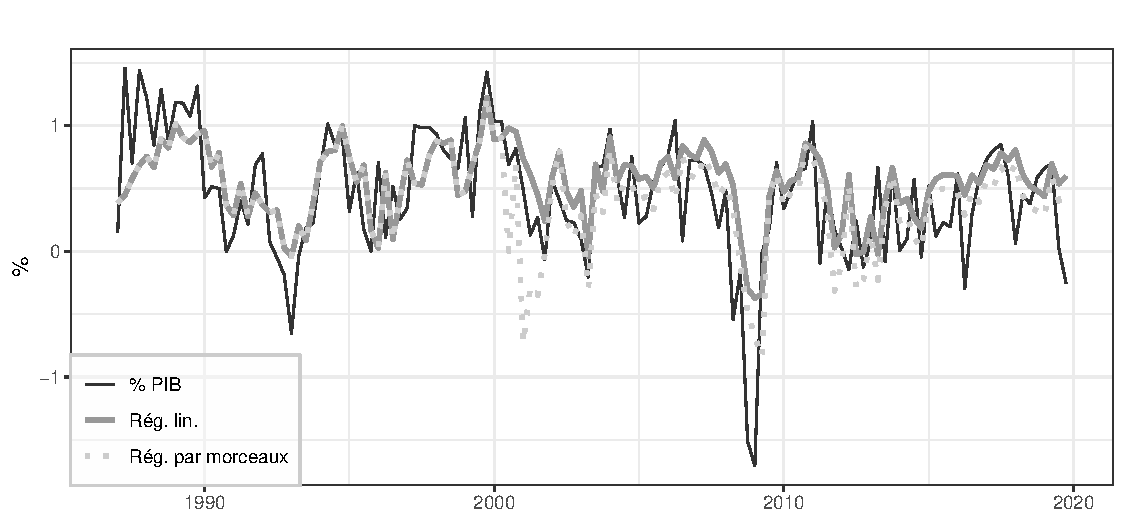
\includegraphics{DT-tvcoef_files/figure-pdf/fig-prev-piecereg-1.pdf}

}

\end{figure}%

Comme indiqué dans la section~\ref{sec-test-baiperron}, l'inconvénient
de cette méthode provient du choix de la date de rupture lorsque
celle-ci n'est pas imposée par l'utilisateur. La
figure~\ref{fig-temps-reel-bp} montre les dates de la rupture détectée
par la procédure de Bai et Perron en fonction de la date de fin de fin
d'estimation du modèle de régression linéaire : aucune rupture n'est
détectée avant 2009 ou lorsque le modèle est estimé en utilisant des
données jusqu'en 2013T2-2015T3. En fonction de la date de fin
d'estimation, la rupture détectée automatiquement peut tout aussi bien
être en 2000 qu'en 2004 ou 2006. Même s'il est possible que cela n'ait
que très peu d'effet sur les prévisions estimées en fin de période,
l'interprétation faite du modèle sera vraisemblablement différente !

\begin{figure}

\caption{\label{fig-temps-reel-bp}Date de rupture détectée par
l'algorithme de Bai et Perron en fonction de la date de fin d'estimation
du modèle.}

\centering{

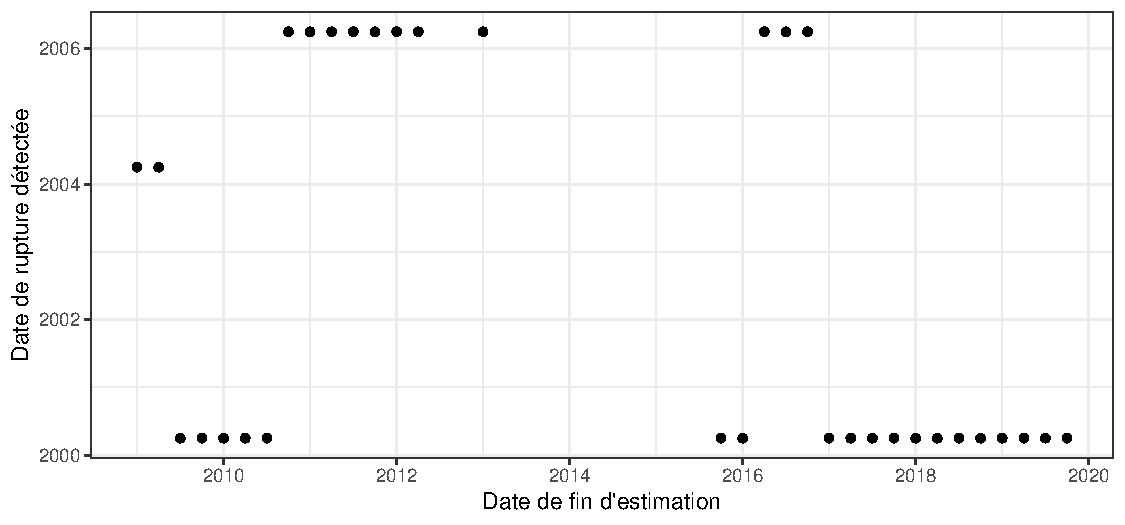
\includegraphics{DT-tvcoef_files/figure-pdf/fig-temps-reel-bp-1.pdf}

}

\end{figure}%

\subsection{De la régression mobile à la régression
locale}\label{sec-reg-locale}

La régression mobile est une des méthodes empiriques les plus simples
pour savoir si les coefficients évoluent dans le temps. Celle-ci
consiste à estimer des régression en utilisant un intervalle de temps
fixe et à observer la courbe des coefficients estimés. En reprenant
notre exemple où les données commencent en 1980, avec une fenêtre fixe
de 15 ans (par exemple), cela consiste à estimer une première régression
entre 1980T1 et 1994T4, une deuxième entre 1980T2 et 1995T1\ldots{} et
une dernière entre 2005T1 et 2019T4. Sous R cela peut par exemple
s'estimer en utilisant la fonction \texttt{roll::roll\_lm()}
\autocite{roll} :

\begin{Shaded}
\begin{Highlighting}[]
\NormalTok{roll\_lm }\OtherTok{\textless{}{-}}\NormalTok{ roll}\SpecialCharTok{::}\FunctionTok{roll\_lm}\NormalTok{(}
  \AttributeTok{x =}\NormalTok{ data\_gdp[, }\FunctionTok{c}\NormalTok{(}\StringTok{"bc\_fr\_m1"}\NormalTok{, }\StringTok{"diff\_bc\_fr\_m1"}\NormalTok{)],}
  \AttributeTok{y =}\NormalTok{ data\_gdp[, }\StringTok{"growth\_gdp"}\NormalTok{],}
  \AttributeTok{width =} \DecValTok{4} \SpecialCharTok{*} \DecValTok{15}
\NormalTok{)}
\NormalTok{coef\_roll\_lm }\OtherTok{\textless{}{-}} \FunctionTok{ts}\NormalTok{(roll\_lm}\SpecialCharTok{$}\NormalTok{coefficients, }\AttributeTok{start =} \DecValTok{1980}\NormalTok{, }\AttributeTok{frequency =} \DecValTok{4}\NormalTok{)}
\end{Highlighting}
\end{Shaded}

La figure~\ref{fig-coef-rollreg} montre les coefficients estimés par
cette régression mobile. Seule ceux estimés sur le climat des affaires
en différence montrent une rupture nette. Elle s'observe à partir de
2009, lorsque plus de la moitié des points de la fenêtre (7,5 ans) sont
estimés après la date de rupture détectée (2000T2).

\begin{figure}

\caption{\label{fig-coef-rollreg}Coefficients estimés par régression
mobile et régression par morceaux.}

\centering{

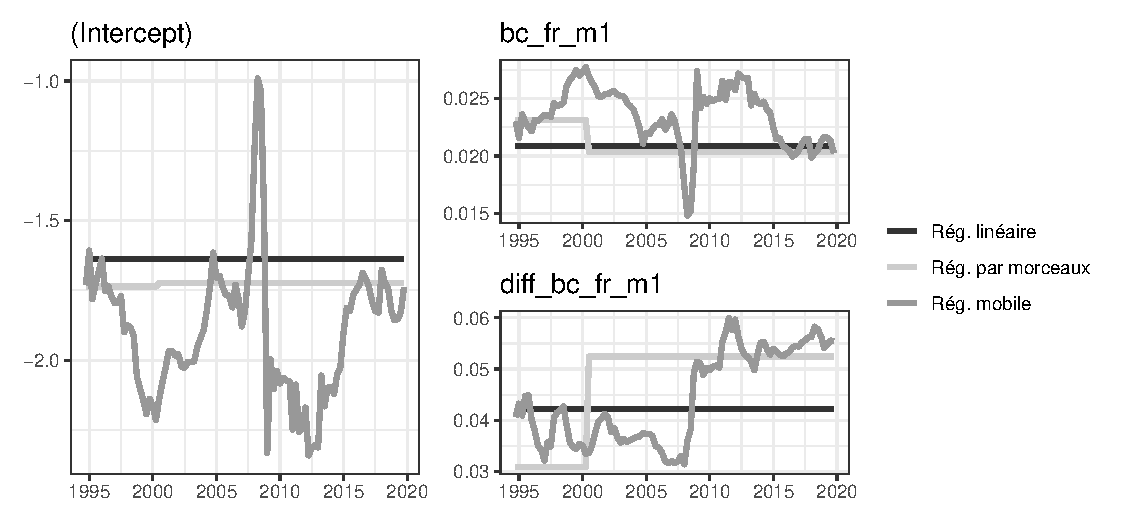
\includegraphics{DT-tvcoef_files/figure-pdf/ffig-coef-rollreg-1.pdf}

Lecture : la régression mobile est estimée sur une fenêtre de 15 ans.
Les coefficients estimés en 1994T4 correspondent aux coefficients
estimés entre 1980T1 et 1994T4.

}

\end{figure}%

La régression mobile a l'avantage d'être très simple mais repose sur
plusieurs paramètres qui ont ici été fixés arbitrairement dont notamment
:

\begin{itemize}
\item
  La longueur de la fenêtre : elle doit être suffisamment large pour
  avoir des bonnes estimations mais suffisamment courte afin de
  permettre de prendre en compte les ruptures.
\item
  La date à laquelle les coefficients sont associés. Dans la fonction
  \texttt{roll::roll\_lm()} ils sont associés à la dernière date de la
  fenêtre : les coefficients de la date \(t\) correspondent à ceux
  obtenus en utilisant les données jusqu'à la date \(t.\) Ils auraient
  également pu être associés à la première date de la fenêtre ou encore
  à son milieu (coefficients de la date \(t\) estimés en utilisant
  autant d'observations avant et après \(t\)). Dans tous les cas une
  stratégie doit être adoptée afin de gérer les observations manquantes
  (dans notre exemple il s'agit donc d'estimer les coefficients avant
  1994).
\end{itemize}

La régression locale permet, grâce à une modélisation plus poussée, de
donner des solutions à ce problème. Dans ce papier nous détaillons la
modélisation utilisée dans la fonction \texttt{tvReg::tvLM()} développée
par \textcite{tvReg}\footnote{ D'autres packages sont disponibles pour
  effectuer de la régression locale, dont par exemple \texttt{locfit} de
  \textcite{locfit}. Toutefois, nous avons ici privilégié le package
  \texttt{tvReg} du fait de sa simplicité d'utilisation et parce qu'il
  implémente également une fonction \texttt{tvReg::tvAR()} pour permet
  de prendre en compte de manière optimale les retards de la variable
  endogène (non étudiée dans cette étude).}. On suppose ici que les
coefficients \(\bf\alpha_t\) dépendent d'une variable aléatoire \(z_t\)
: \(\bf\alpha_t=\alpha(z_t).\) Par défaut \(z_t=t/T\) avec \(T\) le
nombre d'observations : les coefficients dépendent donc d'une mesure
normalisée du temps. On suppose que la fonction \(\alpha\) est
localement constante (\(\alpha(z_t)\simeq \alpha(z)\), option par
défaut) ou localement linéaire
(\(\alpha(z_t)\simeq \alpha(z)+\alpha'(z)(z_t-z)\)), c'est-à-dire que
pour toute date \(t\) on a pour toute date \(i\) proche de \(t\) :
\(\alpha(z_i)\simeq\alpha(z_t)\) ou
\(\alpha(z_i)\simeq\alpha(z_t)+\alpha'(z_t)(z_i-z_t).\) Cette
approximation locale est justifiée par le théorème de Taylor.

Pour chaque date \(t\), le coefficient \(\alpha_t=\alpha(z_t)\) est
obtenu par moindres carrés pondérés. Lorsque \(\alpha\) est supposé
localement constant il s'agit du système : \[
\hat{\bf\alpha_t}=\hat{\alpha}(z_t)=\underset{\bf\theta_0}\argmin\sum_{i=1}^T\left[y_i-{\bf X_i}\bf\theta_0 \right]^2K_{b_t}(z_i-z_t).
\] Lorsque \(\alpha\) est supposé localement linéaire il s'agit du
système : \[
(\hat{\alpha}(z_t), \hat{\alpha}'(z_t))=\underset{\bf \theta_0,\bf \theta_1}\argmin\sum_{i=1}^T\left[y_i-{\bf X_i}\bf\theta_0 - (z_i-z_t){\bf X_i}\bf\theta_1\right]^2K_{b_t}(z_i-z_t).
\] Avec
\(K_{b_t}(z_i-z_t)=\frac{1}{b_t}K\left(\frac{z_i-z_t}{b_t}\right)\) et
\(K(\cdot)\) une fonction de noyau. La fonction \(K\) permet de pondérer
les observations : pour l'estimation du coefficient à la date \(t\) on
accorde généralement plus d'importance (i.e., un poids plus important)
aux observations qui sont proches de \(t\) qu'à celles qui sont
éloignées de \(t.\) C'est une fonction positive, paire et intégrable
telle que \(\int_{-\infty}^{+\infty}K(u) \ud u=1.\) Trois noyaux sont
disponibles dans la fonction \texttt{tvReg::tvLM()} :

\begin{itemize}
\item
  Le cubique (\emph{triweight}, utilisé par défaut) : \[
  K(u)=\frac{35}{32}\left(
  1-
  \left\lvert
  u
  \right\lvert^2
  \right)^3\1_{[-1,1]}(u).
  \]
\item
  Le noyau d'Epanechnikov (ou parabolique) : \[
  K(u)=\frac{3}{4}\left(
  1-
  \left\lvert
  u
  \right\lvert^2
  \right)\1_{[-1,1]}(u).
  \]
\item
  Le noyau Gaussien : \[
  K(u)=\frac{1}{\sqrt{2\pi}}\exp\left(-\frac{1}{2}u^2\right).
  \]
\end{itemize}

Le paramètre \(b_t\) permet de calibrer la largeur de la fenêtre (i.e.,
le nombre de points utilisés pour chaque estimation). Il est
généralement supposé constant (\(b_t=b\)).

Dans notre exemple de prévision du PIB, \(T=160\) observations sont
utilisées. Avec \(z_t=t/T\) et indexant chaque observation entre 1 et
\(T,\) la régression mobile sur 15 ans où l'on affecte le coefficient de
la date \(t\) au milieu de la fenêtre d'estimation est donc retrouvée en
utilisant le noyau uniforme \(K(u)=\1_{[-1,1]}(x)\) avec
\(b_t=b=\frac{30}{160}.\) En effet, dans ce cas \(K(z_t-z_i)\ne0\) si et
seulement si \(|t-i|\leq30\) : on utilise donc 30 observations (soit
\(7,5\) ans) autour de \(t\) pour estimer le coefficient à la date
\(t.\)

Dans \texttt{tvReg}, le paramètre \(b\) est par défaut obtenu en
minimisant une statistique de validation croisée dans l'intervalle
\(\left[\frac{5}{T},20\right].\) Lorsque \(b\) est plus grand que 1,
toutes les observations sont utilisées pour l'estimation de chaque
coefficient \(\bf\alpha_t.\) Plus \(b\) se rapproche de 1 plus on se
rapproche du cas de la régression linéaire puisque dans ce cas les poids
donnés par \(K\) tendent à être constants pour toutes les observations.
En effet, dans ce cas, pour \(T=160,\)
\(\frac{\max_u K(u)}{\min_u K(u)}\) est compris entre \(1,001\) et
\(1,008\) pour les noyaux cubiques, paraboliques et gaussiens.

Reprenons notre exemple de prévision du PIB avec une détection
automatique de la fenêtre.

\begin{Shaded}
\begin{Highlighting}[]
\NormalTok{reg\_loc }\OtherTok{\textless{}{-}}\NormalTok{ tvReg}\SpecialCharTok{::}\FunctionTok{tvLM}\NormalTok{(}
  \AttributeTok{formula =}\NormalTok{ growth\_gdp }\SpecialCharTok{\textasciitilde{}}\NormalTok{ bc\_fr\_m1 }\SpecialCharTok{+}\NormalTok{ diff\_bc\_fr\_m1,}
  \AttributeTok{data =}\NormalTok{ data\_gdp}
\NormalTok{)}
\end{Highlighting}
\end{Shaded}

\begin{verbatim}
Calculating regression bandwidth... bw =  0.7485784 
\end{verbatim}

\begin{Shaded}
\begin{Highlighting}[]
\FunctionTok{summary}\NormalTok{(reg\_loc)}
\end{Highlighting}
\end{Shaded}

\begin{verbatim}

Call: 
tvReg::tvLM(formula = growth_gdp ~ bc_fr_m1 + diff_bc_fr_m1, 
    data = data_gdp)

Class:  tvlm 

Summary of time-varying estimated coefficients: 
================================================ 
        (Intercept) bc_fr_m1 diff_bc_fr_m1
Min.         -1.924  0.02037       0.03429
1st Qu.      -1.886  0.02145       0.03930
Median       -1.800  0.02233       0.04470
Mean         -1.773  0.02222       0.04342
3rd Qu.      -1.680  0.02308       0.04777
Max.         -1.503  0.02338       0.04927

Bandwidth:  0.7486
Pseudo R-squared:  0.4549 
\end{verbatim}

La fenêtre estimée par défaut est de 0,75, c'est-à-dire que pour estimer
le coefficient à la date \(t\) on utilise au plus 30 ans avant et après
\(t\) : on utilise tous les points dans la majorité des cas. Cela
explique le caractère très lisse des coefficients
(figure~\ref{fig-coef-reg-mobile}). Avec ce paramètre pour la fenêtre,
les ruptures brutales sont donc difficiles à prendre en compte.

\begin{figure}

\caption{\label{fig-coef-reg-mobile}Coefficients estimés par régression
linéaire, régression par morceaux et régression locale (avec
\(b=0,74\)).}

\centering{

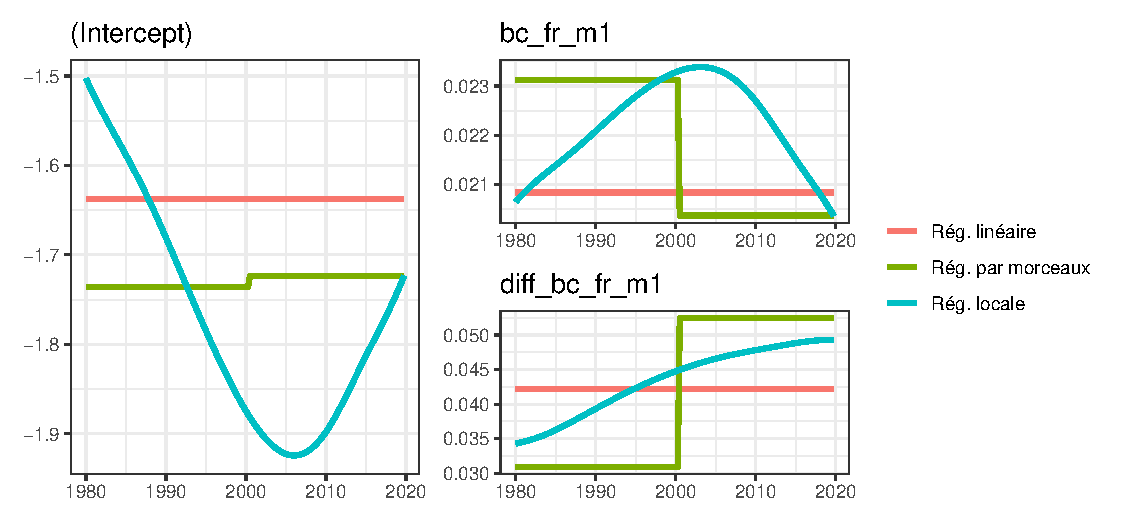
\includegraphics{DT-tvcoef_files/figure-pdf/fig-coef-reg-mobile-1.pdf}

}

\end{figure}%

Un des inconvénients de méthode de sélection automatique de la fenêtre
est que la statistique de validation croisée est un critère peu
discriminant (voir \textcite{Loader1999}) : il peut y avoir très peu de
différences entre différentes valeurs de la fenêtre alors que celle-ci a
un impact fort sur l'interprétation du modèle ! Cela a également pour
effet que la méthode est peu stable dans le temps
(figure~\ref{fig-oos-bw}), ce qui augmente les sources de révisions des
simulations hors échantillon, calculables en utilisant la fonction
\texttt{oos\_prev()} :

\begin{Shaded}
\begin{Highlighting}[]
\NormalTok{oos\_reg\_loc }\OtherTok{\textless{}{-}} \FunctionTok{oos\_prev}\NormalTok{(reg\_loc)}
\NormalTok{oos\_bw }\OtherTok{\textless{}{-}} \FunctionTok{ts}\NormalTok{(}\FunctionTok{sapply}\NormalTok{(oos\_reg\_loc}\SpecialCharTok{$}\NormalTok{model, }\StringTok{\textasciigrave{}}\AttributeTok{[[}\StringTok{\textasciigrave{}}\NormalTok{,}\StringTok{"bw"}\NormalTok{),}
             \AttributeTok{end =} \FunctionTok{c}\NormalTok{(}\DecValTok{2019}\NormalTok{, }\DecValTok{4}\NormalTok{),}
             \AttributeTok{frequency =} \DecValTok{4}\NormalTok{)}
\end{Highlighting}
\end{Shaded}

\begin{verbatim}
Scale for x is already present.
Adding another scale for x, which will replace the existing scale.
\end{verbatim}

\begin{figure}

\caption{\label{fig-oos-bw}Fenêtre \(b\) détectée automatiquement en
fonction de la date de fin d'estimation du modèle.}

\centering{

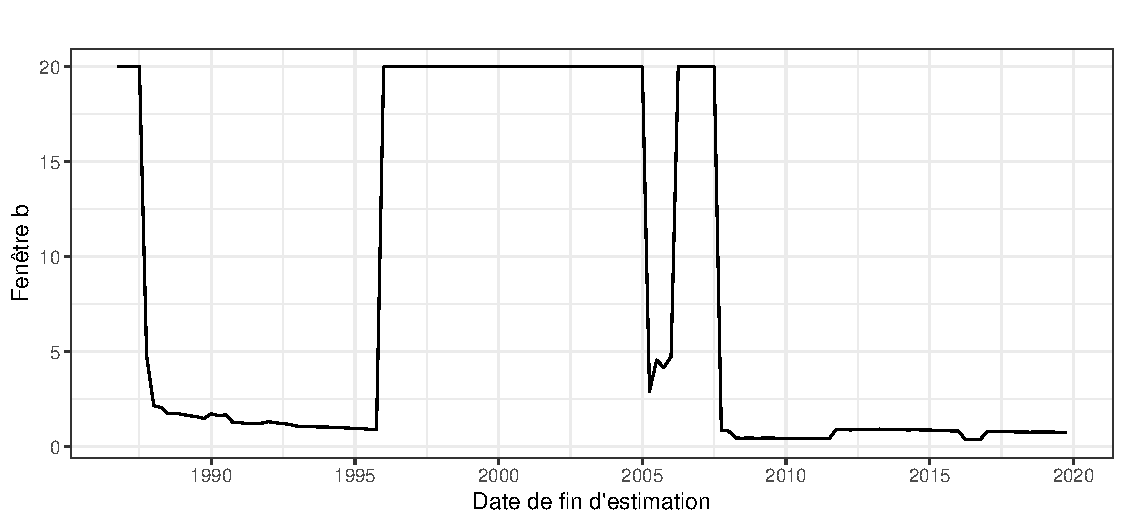
\includegraphics{DT-tvcoef_files/figure-pdf/fig-oos-bw-1.pdf}

}

\end{figure}%

Pour l'estimation hors échantillon, la méthode utilisée est
l'utilisation d'une fonction de noyau tronquée : plus de points dans le
passé que dans le futur sont utilisés pour estimer les derniers
coefficients. C'est donc également une source de révision au fur et à
mesure que des nouveaux points seront connus. Même si des méthodes
optimales existent pour minimiser les erreurs d'estimation des
coefficients hors échantillon (voir par exemple
\textcite{FengSchafer2021}), cela devrait ici avoir peu d'impact car un
modèle très simple est ici utilisé pour estimer les coefficients
(approximation de la fonction \(\alpha\) par une constante).

Un autre inconvénient de ces méthodes est que tous les coefficients
varient dans la temps alors que dans certains cas on peut supposer la
relation constante. Si l'on souhaite fixer certains coefficients, on
peut procéder comme dans la section~\ref{sec-test-baiperron} en faisant
une régression linéaire, pour estimer les coefficients fixes, suivie
d'une régression mobile.

\subsection{Modélisation espace-état}\label{sec-ssm}

La modélisation espace-état est une méthodologie générale permettant de
traiter un grand nombre de problèmes de séries temporelles. Dans cette
approche, on suppose que tout modèle est déterminé par une série de
vecteurs non observés \(\alpha_1,\dots,\alpha_n\) associés aux
observations \(y_1,\dots,y_n\), la relation entre \(\alpha_t\) et
\(y_t\) étant spécifiée par le modèle espace-état. Ces modèles sont
largement décrits dans la littérature, notamment par
\textcite{durbinkoopman}. Dans cet article, nous nous placerons dans un
cadre simplifié des modèles linéaires gaussiens appliqués aux
régressions linéaires. Les modèles sont déterminés par un ensemble de
deux équations : \[
\begin{cases}
y_t={\bf X_t}\bf\alpha_t+\varepsilon_t,\quad&\varepsilon_t\sim\mathcal N(0,\sigma^2)\\
\bf\alpha_{t+1}=\bf\alpha_t+\bf\eta_t,\quad&\bf\eta_t\sim\mathcal N(\bf 0,\bf\Sigma)
\end{cases},\text{ avec }\eta_t\text{ et }\varepsilon_t\text{ indépendants.}
\] La première équation est l'équation d'observation (\emph{observation
equation}), la seconde l'équation d'état (\emph{state equation}) et
\(\bf\alpha_t\) le vecteur d'états (\emph{state vector}).

Dans cette étude, la matrice de variance-covariance \(\bf\Sigma\) est
supposée diagonale : la dynamique d'évolution des coefficients d'une
variable est donc indépendante de la dynamique d'évolution des autres
variables. Lorsque des contraintes entre les différents coefficients
existent, des spécifications différentes de la matrice de
variance-covariance \(\bf\Sigma\) peuvent être faites : c'est par
exemple ce qui a été fait par \textcite{abs2006} pour estimer des
coefficients jours ouvrables variant dans le temps. On retrouve le cas
de la régression linéaire lorsque \(\bf\Sigma=\bf 0\) puisque dans ce
cas tous les \(\alpha_t\) sont égaux.

Ces modèles sont implémentés dans la fonction \texttt{tvCoef::ssm\_lm()}
qui prend en entrée un modèle de régression linéaire. L'implémentation
est basée sur le package \texttt{rjd3sts} \autocite{rjd3sts} qui permet
d'implémenter très facilement les modèles espaces-état sans devoir
écrire explicitement le modèle. Par défaut les variances du vecteur
d'états (\(\bf \Sigma\)) ne sont pas estimés et fixés à 0 : on retrouve
donc les coefficients estimés par régression linéaire.

\begin{Shaded}
\begin{Highlighting}[]
\NormalTok{ssm }\OtherTok{\textless{}{-}} \FunctionTok{ssm\_lm}\NormalTok{(reg\_lin)}
\NormalTok{ssm}
\end{Highlighting}
\end{Shaded}

\begin{verbatim}
Mean of time-varying estimated coefficients (smoothing): 
  (Intercept)      bc_fr_m1 diff_bc_fr_m1         noise 
      -1.6377        0.0208        0.0422        0.0000 
\end{verbatim}

L'estimation des hyperparamètres (variances des bruits blancs) est faite
par maximum de vraisemblance différentes méthodes existent pour
initialiser les modèles (calculer \(\bf \alpha_1\)). Pour plus de
détails voir par exemple \textcite{durbinkoopman}. Le filtre de Kalman
permet ensuite de calculer tous les coefficients. Parmi les paramètres
calculés, les deux principaux sont :

\begin{enumerate}
\def\labelenumi{\arabic{enumi}.}
\tightlist
\item
  Les états lissés (\emph{smoothed states})
  \(\E{\alpha_t|y_1,\dots,y_n}\) : il s'agit de l'estimation des états
  (\(\bf\alpha_t\)) en utilisant toute l'information disponible. Dans le
  cadre de la régression linéaire, les états lissés sont donc constants
  sur toutes les dates et correspondent aux coefficients estimés en
  utilisant l'ensemble des données disponibles :
\end{enumerate}

\begin{Shaded}
\begin{Highlighting}[]
\FunctionTok{window}\NormalTok{(ssm}\SpecialCharTok{$}\NormalTok{smoothed\_states, }\AttributeTok{start =} \DecValTok{2019}\NormalTok{)}
\end{Highlighting}
\end{Shaded}

\begin{verbatim}
        (Intercept)   bc_fr_m1 diff_bc_fr_m1       noise
2019 Q1   -1.637698 0.02084469    0.04215106  0.23277648
2019 Q2   -1.637698 0.02084469    0.04215106  0.01219046
2019 Q3   -1.637698 0.02084469    0.04215106 -0.50526528
2019 Q4   -1.637698 0.02084469    0.04215106 -0.84723791
\end{verbatim}

\begin{enumerate}
\def\labelenumi{\arabic{enumi}.}
\setcounter{enumi}{1}
\tightlist
\item
  Les états filtrés (\emph{filtered states})
  \(\E{\alpha_t|y_1,\dots,y_{t-1}}\) : il s'agit de l'estimation des
  états (\(\bf\alpha_t\)) en utilisant l'information disponible jusqu'à
  la date précédente. Dans le cadre de la régression linéaire, cela
  correspond aux coefficients estimés hors échantillon : la valeur des
  états filtrés en 2010T2 correspond aux coefficients estimés en
  utilisant les données jusqu'au 2010T1. Ils permettent donc d'avoir une
  estimation des prévisions hors échantillon du modèle.
\end{enumerate}

\begin{Shaded}
\begin{Highlighting}[]
\FunctionTok{round}\NormalTok{(}\FunctionTok{window}\NormalTok{(ssm}\SpecialCharTok{$}\NormalTok{filtering\_states, }\AttributeTok{start =} \FunctionTok{c}\NormalTok{(}\DecValTok{2010}\NormalTok{, }\DecValTok{2}\NormalTok{), }\AttributeTok{end =} \FunctionTok{c}\NormalTok{(}\DecValTok{2010}\NormalTok{, }\DecValTok{2}\NormalTok{)), }\DecValTok{6}\NormalTok{)}
\end{Highlighting}
\end{Shaded}

\begin{verbatim}
        (Intercept) bc_fr_m1 diff_bc_fr_m1 noise
2010 Q2   -1.733678 0.022248       0.04724     0
\end{verbatim}

\begin{Shaded}
\begin{Highlighting}[]
\FunctionTok{round}\NormalTok{(}\FunctionTok{coef}\NormalTok{(}\FunctionTok{dynlm}\NormalTok{(}
  \AttributeTok{formula =}\NormalTok{ growth\_gdp }\SpecialCharTok{\textasciitilde{}}\NormalTok{ bc\_fr\_m1 }\SpecialCharTok{+}\NormalTok{ diff\_bc\_fr\_m1,}
  \AttributeTok{data =} \FunctionTok{window}\NormalTok{(gdp, }\AttributeTok{start =} \DecValTok{1980}\NormalTok{, }\AttributeTok{end =} \FunctionTok{c}\NormalTok{(}\DecValTok{2010}\NormalTok{,}\DecValTok{1}\NormalTok{))}
\NormalTok{)), }\DecValTok{6}\NormalTok{)}
\end{Highlighting}
\end{Shaded}

\begin{verbatim}
  (Intercept)      bc_fr_m1 diff_bc_fr_m1 
    -1.733678      0.022248      0.047240 
\end{verbatim}

Lorsque les variances sont estimées, les états filtrés ne correspondent
pas à exactement à des estimations hors échantillon car les
hyperparamètres sont fixés (variances \(\bf\Sigma\) et initialisation).
Les estimations hors échantillon peuvent être calculées en utilisant la
fonction \texttt{tvCoef::ssm\_lm\_oos()}.

Pour faciliter l'estimation des variances \(\bf\Sigma,\) le paramètre
est souvent reparamétré : \[
\begin{cases}
y_t={\bf X_t}\bf\alpha_t+\varepsilon_t,\quad&\varepsilon_t\sim\mathcal N(0,\sigma^2)\\
\bf\alpha_{t+1}=\bf\alpha_t+\bf\eta_t,\quad&\bf\eta_t\sim\mathcal N(\bf 0,\sigma^2\bf Q)
\end{cases},\text{ avec }\eta_t\text{ et }\varepsilon_t\text{ indépendants.}
\] Les variances sont donc définies à un facteur multiplicatif près et
une estimation en deux étapes est faite : la vraisemblance est dite
\emph{concentrée}. C'est ce qui est utilisé par défaut dans
\texttt{tvCoef::ssm\_lm()}. Dans notre exemple, l'erreur standard de la
régression (\emph{residual standar error}) peut se calculer de la façon
suivante :

\begin{Shaded}
\begin{Highlighting}[]
\FunctionTok{sqrt}\NormalTok{(ssm}\SpecialCharTok{$}\NormalTok{parameters}\SpecialCharTok{$}\NormalTok{parameters }\SpecialCharTok{*}\NormalTok{ ssm}\SpecialCharTok{$}\NormalTok{parameters}\SpecialCharTok{$}\NormalTok{scaling)}
\end{Highlighting}
\end{Shaded}

\begin{verbatim}
(Intercept).var       noise.var 
      0.0000000       0.3757355 
\end{verbatim}

\begin{Shaded}
\begin{Highlighting}[]
\FunctionTok{summary}\NormalTok{(reg\_lin)}\SpecialCharTok{$}\NormalTok{sigma}
\end{Highlighting}
\end{Shaded}

\begin{verbatim}
[1] 0.3757355
\end{verbatim}

Afin d'estimer les variances associées à l'équation d'état, il faut
utiliser les paramètres \texttt{fixed\_var\_intercept\ =\ FALSE} et
\texttt{fixed\_var\_trend\ =\ FALSE}. Même si la valeur des variances
(\texttt{var\_intercept} et \texttt{var\_variables} qui valent 0 par
défaut) n'aura aucun effet sur les variances finales estimées, il est
parfois nécessaire de modifier ces valeurs afin d'éviter une erreur dans
l'optimisation. Sur notre modèle, l'optimisation conduit à garder fixe
le coefficient associé au climat des affaires en niveau (variance nulle)
mais considère que les autres variables varient dans le temps :

\begin{Shaded}
\begin{Highlighting}[]
\NormalTok{ssm }\OtherTok{\textless{}{-}} \FunctionTok{ssm\_lm}\NormalTok{(reg\_lin, }
              \AttributeTok{fixed\_var\_intercept =} \ConstantTok{FALSE}\NormalTok{, }
              \AttributeTok{fixed\_var\_variables =} \ConstantTok{FALSE}\NormalTok{)}
\FunctionTok{sqrt}\NormalTok{(ssm}\SpecialCharTok{$}\NormalTok{parameters}\SpecialCharTok{$}\NormalTok{parameters }\SpecialCharTok{*}\NormalTok{ ssm}\SpecialCharTok{$}\NormalTok{parameters}\SpecialCharTok{$}\NormalTok{scaling)}
\end{Highlighting}
\end{Shaded}

\begin{verbatim}
  (Intercept).var      bc_fr_m1.var diff_bc_fr_m1.var         noise.var 
      0.019564504       0.000000000       0.009305432       0.335063783 
\end{verbatim}

\begin{remark}
Dans la version actuelle de \texttt{tvCoef}, les retards de la variable
endogène (à prévoir) ne sont pas modélisés correctement. En effet, dans
ce cas il faudrait utiliser une modélisation différente afin de prendre
en compte la relation entre la variable endogène et les retards.
\end{remark}

La figure~\ref{fig-coef-ssm} montre les coefficients estimés avec toutes
les méthodes présentées dans ce papier. Pour toutes les méthodes, le
coefficient du climat des affaires en niveau est stable dans le temps
(coefficients estimés compris entre 0,020 et 0,023). En revanche, les
résultats du modèle espace-état sont sensiblement différents pour le
coefficient associé au climat des affaires, avec des périodes où le
coefficient est plus faible que pour les autres méthodes (avant 1983,
entre 1995 et 1999 et après 2011) et d'autres où il est plus élevé
(notamment pendant la crise financière).

\begin{figure}

\caption{\label{fig-coef-ssm}Coefficients estimés par régression
linéaire, régression par morceaux, régression locale (avec \(b=0,74\))
et modèle espace-état.}

\centering{

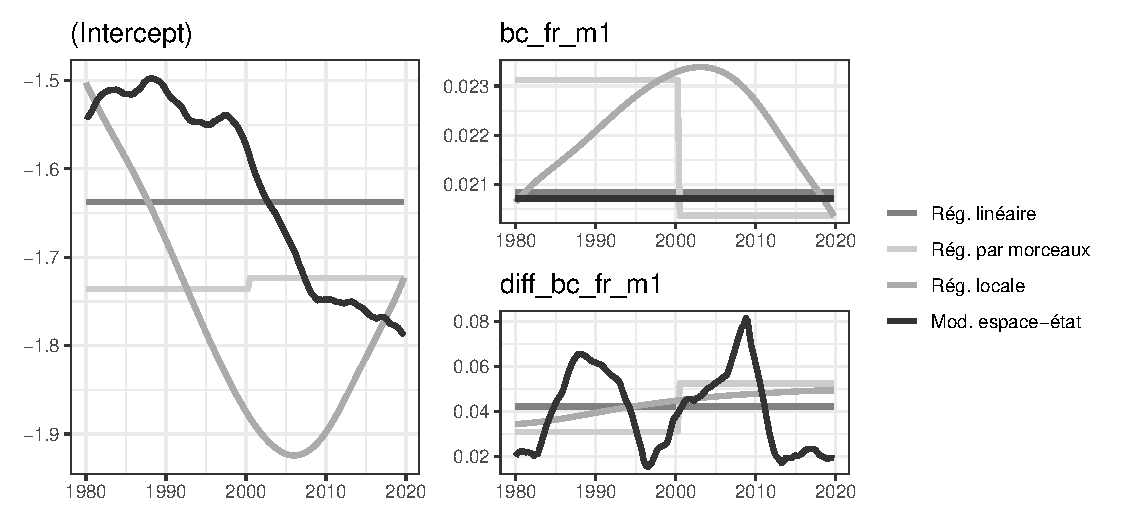
\includegraphics{DT-tvcoef_files/figure-pdf/fig-coef-ssm-1.pdf}

}

\end{figure}%

La table~\ref{tbl-res-model-pib} compare la qualité prédictive des
différents modèles dans l'échantillon (en utilisant toutes les données
et pour estimer les paramètres des modèles) et hors échantillon
(reproduction du processus de prévision en estimant, de manière
récursive les modèles jusqu'à la date \(t\) pour calculer les prévisions
à la date \(t+1\)). C'est la modélisation espace-état qui minimise les
erreurs de prévision, suivie de la régression par morceaux. La
régression locale a une erreur hors échantillon plus élevée notamment du
fait des instabilités sur l'estimation de la fenêtre. Le test de
Diebold-Mariano (voir notamment \textcite{DMtest}), implémenté dans la
fonction \texttt{forecast::dm.test()} \autocite{forecastR}, permet de
tester si cette différence est significative. Dans et hors échantillon,
les modèles espace-état ont des erreurs de prévisions significativement
plus petites que la régression linéaire (p-valeurs respectivement de
0,00 et 0,05). Dans l'échantillon elles sont également significativement
plus petites que celles de la régression par morceau (p-valeur de 0,00)
mais la différence n'est pas significative hors échantillon (p-valeur de
0,10) : l'interprétation économique sur les périodes récentes est en
revanche différente (coefficient sur le climat des affaires en
différence), ce qui conduit donc à des prévisions différentes.

\begin{Shaded}
\begin{Highlighting}[]
\NormalTok{oos\_ssm }\OtherTok{\textless{}{-}} \FunctionTok{ssm\_lm\_oos}\NormalTok{(reg\_lin, }\AttributeTok{fixed\_var\_intercept =} \ConstantTok{FALSE}\NormalTok{, }
                      \AttributeTok{fixed\_var\_variables =} \ConstantTok{FALSE}\NormalTok{,}
                      \AttributeTok{date =} \DecValTok{70}\NormalTok{)}

\NormalTok{res\_is }\OtherTok{\textless{}{-}} \FunctionTok{ts.union}\NormalTok{(}
  \FunctionTok{ts}\NormalTok{(}\FunctionTok{residuals}\NormalTok{(reg\_lin), }\AttributeTok{end =} \FunctionTok{c}\NormalTok{(}\DecValTok{2019}\NormalTok{,}\DecValTok{4}\NormalTok{), }\AttributeTok{frequency =} \DecValTok{4}\NormalTok{),}
  \FunctionTok{residuals}\NormalTok{(reg\_morc),}
  \FunctionTok{ts}\NormalTok{(}\FunctionTok{residuals}\NormalTok{(reg\_loc), }\AttributeTok{end =} \FunctionTok{c}\NormalTok{(}\DecValTok{2019}\NormalTok{,}\DecValTok{4}\NormalTok{), }\AttributeTok{frequency =} \DecValTok{4}\NormalTok{),}
  \FunctionTok{residuals}\NormalTok{(ssm)[,}\StringTok{"smoothed"}\NormalTok{]}
\NormalTok{)}
\NormalTok{res\_oos }\OtherTok{\textless{}{-}} \FunctionTok{ts.union}\NormalTok{(}
\NormalTok{  oos\_lm}\SpecialCharTok{$}\NormalTok{residuals,}
\NormalTok{  oos\_reg\_morc}\SpecialCharTok{$}\NormalTok{residuals,}
  \FunctionTok{ts}\NormalTok{(oos\_reg\_loc}\SpecialCharTok{$}\NormalTok{residuals, }\AttributeTok{end =} \FunctionTok{c}\NormalTok{(}\DecValTok{2019}\NormalTok{,}\DecValTok{4}\NormalTok{), }\AttributeTok{frequency =} \DecValTok{4}\NormalTok{),}
\NormalTok{  oos\_ssm}\SpecialCharTok{$}\NormalTok{oos\_noise}
\NormalTok{)}
\NormalTok{res\_oos }\OtherTok{\textless{}{-}} \FunctionTok{window}\NormalTok{(res\_oos, }\AttributeTok{start =} \DecValTok{2003}\NormalTok{)}
\CommentTok{\# (H0) : Modèle espace{-}état meilleur que modèle linéaire}
\NormalTok{forecast}\SpecialCharTok{::}\FunctionTok{dm.test}\NormalTok{(res\_is[, }\DecValTok{1}\NormalTok{], res\_is[, }\DecValTok{4}\NormalTok{], }\StringTok{"greater"}\NormalTok{)}
\end{Highlighting}
\end{Shaded}

\begin{verbatim}

    Diebold-Mariano Test

data:  res_is[, 1]res_is[, 4]
DM = 3.3521, Forecast horizon = 1, Loss function power = 2, p-value =
0.0005012
alternative hypothesis: greater
\end{verbatim}

\begin{Shaded}
\begin{Highlighting}[]
\CommentTok{\# (H0) : Modèle espace{-}état meilleur que régression par morceaux}
\NormalTok{forecast}\SpecialCharTok{::}\FunctionTok{dm.test}\NormalTok{(res\_is[, }\DecValTok{2}\NormalTok{], res\_is[, }\DecValTok{4}\NormalTok{], }\StringTok{"greater"}\NormalTok{)}
\end{Highlighting}
\end{Shaded}

\begin{verbatim}

    Diebold-Mariano Test

data:  res_is[, 2]res_is[, 4]
DM = 3.2101, Forecast horizon = 1, Loss function power = 2, p-value =
0.0008026
alternative hypothesis: greater
\end{verbatim}

\begin{Shaded}
\begin{Highlighting}[]
\CommentTok{\# (H0) : Modèle espace{-}état meilleur que modèle linéaire}
\NormalTok{forecast}\SpecialCharTok{::}\FunctionTok{dm.test}\NormalTok{(res\_oos[, }\DecValTok{1}\NormalTok{], res\_oos[, }\DecValTok{4}\NormalTok{], }\StringTok{"greater"}\NormalTok{)}
\end{Highlighting}
\end{Shaded}

\begin{verbatim}

    Diebold-Mariano Test

data:  res_oos[, 1]res_oos[, 4]
DM = 1.6374, Forecast horizon = 1, Loss function power = 2, p-value =
0.05312
alternative hypothesis: greater
\end{verbatim}

\begin{Shaded}
\begin{Highlighting}[]
\CommentTok{\# (H0) : Modèle espace{-}état meilleur que régression par morceaux}
\NormalTok{forecast}\SpecialCharTok{::}\FunctionTok{dm.test}\NormalTok{(res\_oos[, }\DecValTok{2}\NormalTok{], res\_oos[, }\DecValTok{4}\NormalTok{], }\StringTok{"greater"}\NormalTok{)}
\end{Highlighting}
\end{Shaded}

\begin{verbatim}

    Diebold-Mariano Test

data:  res_oos[, 2]res_oos[, 4]
DM = 1.2706, Forecast horizon = 1, Loss function power = 2, p-value =
0.1041
alternative hypothesis: greater
\end{verbatim}

\begin{longtable}[]{@{}lrr@{}}

\caption{\label{tbl-res-model-pib}Erreurs quadratiques moyennes des
erreurs de prévisions entre les différentes méthodes.}

\tabularnewline

\toprule\noalign{}
& Dans l'échantillon & Hors échantillon \\
\midrule\noalign{}
\endhead
\bottomrule\noalign{}
\endlastfoot
Régression linéaire & 0,37 & 0,42 \\
Régression par morceaux & 0,35 & 0,39 \\
Régression locale & 0,35 & 0,41 \\
Modèle espace-état & 0,32 & 0,37 \\

\end{longtable}

Note : Les prévisions dans l'échantillon sont calculées en estimant les
modèles à partir des données disponibles entre 1980T1 et 2019T4. Les
prévisions hors échantillon sont calculées en à partir de 2003T1 : la
première prévision (2003T1) correspond à celle que l'on aurait eu en
estimant les modèles à partir des données disponibles jusqu'en 2002T4
(trimestre précédente).

\subsection{Prise en compte de la période du COVID-19 et
prévision}\label{prise-en-compte-de-la-puxe9riode-du-covid-19-et-pruxe9vision}

Dans les sections précédentes, les modèles ont été estimés jusqu'en
2019T4 dans le but de simplifier la présentation des modèles. Toutefois,
si l'on veut effectuer de la prévision sur les périodes récentes, il est
indispensable de prendre en compte la période du COVID-19. Cela se fait
généralement en ajoutant, dans le modèle de prévision, des variables
explicatives modélisant les chocs de cette période. La méthode la plus
simple consiste à ajouter des indicatrices sur les trimestres concernés
(ici l'année 2020) :

\begin{Shaded}
\begin{Highlighting}[]
\NormalTok{ind }\OtherTok{\textless{}{-}} \FunctionTok{cbind}\NormalTok{(}\FunctionTok{time}\NormalTok{(gdp) }\SpecialCharTok{==} \DecValTok{2020}\NormalTok{, }\FunctionTok{time}\NormalTok{(gdp) }\SpecialCharTok{==} \FloatTok{2020.25}\NormalTok{, }
             \FunctionTok{time}\NormalTok{(gdp) }\SpecialCharTok{==} \FloatTok{2020.5}\NormalTok{, }\FunctionTok{time}\NormalTok{(gdp) }\SpecialCharTok{==} \FloatTok{2020.75}\NormalTok{)}
\NormalTok{ind }\OtherTok{\textless{}{-}} \FunctionTok{ts}\NormalTok{(}\FunctionTok{apply}\NormalTok{(ind,}\DecValTok{2}\NormalTok{, as.numeric), }\AttributeTok{start =} \FunctionTok{start}\NormalTok{(gdp), }\AttributeTok{frequency =} \DecValTok{4}\NormalTok{)}
\FunctionTok{colnames}\NormalTok{(ind) }\OtherTok{\textless{}{-}} \FunctionTok{sprintf}\NormalTok{(}\StringTok{"ind2020T\%i"}\NormalTok{, }\DecValTok{1}\SpecialCharTok{:}\DecValTok{4}\NormalTok{)}
\NormalTok{data\_covid }\OtherTok{\textless{}{-}} \FunctionTok{ts.union}\NormalTok{(gdp, ind)}
\FunctionTok{colnames}\NormalTok{(data\_covid) }\OtherTok{\textless{}{-}} \FunctionTok{c}\NormalTok{(}\FunctionTok{colnames}\NormalTok{(gdp), }\FunctionTok{colnames}\NormalTok{(ind))}

\NormalTok{reg\_lin\_covid }\OtherTok{\textless{}{-}} \FunctionTok{dynlm}\NormalTok{(}
  \AttributeTok{formula =}\NormalTok{ growth\_gdp }\SpecialCharTok{\textasciitilde{}}\NormalTok{ bc\_fr\_m1 }\SpecialCharTok{+}\NormalTok{ diff\_bc\_fr\_m1 }\SpecialCharTok{+}
\NormalTok{    ind2020T1 }\SpecialCharTok{+}\NormalTok{ ind2020T2 }\SpecialCharTok{+}\NormalTok{ ind2020T3 }\SpecialCharTok{+}\NormalTok{ ind2020T4,}
  \AttributeTok{data =} \FunctionTok{window}\NormalTok{(data\_covid, }\AttributeTok{start =} \DecValTok{1980}\NormalTok{)}
\NormalTok{)}
\FunctionTok{coef}\NormalTok{(reg\_lin\_covid)}
\end{Highlighting}
\end{Shaded}

\begin{verbatim}
  (Intercept)      bc_fr_m1 diff_bc_fr_m1     ind2020T1     ind2020T2 
  -1.62422153    0.02075517    0.05366003   -6.14116779   -9.77551672 
    ind2020T3     ind2020T4 
  15.88744163   -1.13892410 
\end{verbatim}

Pour la construction des autres modèles, nous gardons les paramètres
estimés en utilisant les données avant la période du COVID-19, cette
dernière pouvant biaiser les résultats. Ainsi :

\begin{itemize}
\tightlist
\item
  Pour la régression par morceaux, la date de rupture retenue est
  toujours 2000T2 (contre 2016T1 en utilisant les données après 2020).
\item
  Pour la régression locale, la fenêtre utilisée est 0,75 (contre 0,04
  en utilisant les données après 2020).
\item
  Pour la modélisation espace-état, le coefficient du climat des
  affaires en niveau est toujours considéré comme fixe (il est considéré
  comme mobile en utilisant les données après 2020). Toutefois les
  variances des autres coefficients sont de nouveau estimées.
\end{itemize}

\begin{Shaded}
\begin{Highlighting}[]
\CommentTok{\# Date différente de rupture détectée mais l\textquotesingle{}on garde 2000T2 par continuité}
\NormalTok{bp\_covid }\OtherTok{\textless{}{-}} \FunctionTok{breakpoints}\NormalTok{(reg\_lin\_covid)}
\FunctionTok{c}\NormalTok{(}\FunctionTok{breakdates}\NormalTok{(bp), }\FunctionTok{breakdates}\NormalTok{(bp\_covid))}
\end{Highlighting}
\end{Shaded}

\begin{verbatim}
[1] 2000.25 2016.00
\end{verbatim}

\begin{Shaded}
\begin{Highlighting}[]
\NormalTok{bw\_covid }\OtherTok{\textless{}{-}} \FunctionTok{bw}\NormalTok{(}\FunctionTok{window}\NormalTok{(}
\NormalTok{  data\_covid[, }\FunctionTok{c}\NormalTok{(}\StringTok{"bc\_fr\_m1"}\NormalTok{, }\StringTok{"diff\_bc\_fr\_m1"}\NormalTok{, }\StringTok{"ind2020T1"}\NormalTok{, }\StringTok{"ind2020T2"}\NormalTok{, }
                \StringTok{"ind2020T3"}\NormalTok{, }\StringTok{"ind2020T4"}\NormalTok{)], }\AttributeTok{start =} \DecValTok{1980}\NormalTok{, }\AttributeTok{end =} \FunctionTok{c}\NormalTok{(}\DecValTok{2022}\NormalTok{, }\DecValTok{4}\NormalTok{)), }
  \FunctionTok{window}\NormalTok{(data\_covid[, }\StringTok{"growth\_gdp"}\NormalTok{], }\AttributeTok{start =} \DecValTok{1980}\NormalTok{, }\AttributeTok{end =} \FunctionTok{c}\NormalTok{(}\DecValTok{2022}\NormalTok{, }\DecValTok{4}\NormalTok{))}
\NormalTok{  )}
\FunctionTok{c}\NormalTok{(reg\_loc}\SpecialCharTok{$}\NormalTok{bw, bw\_covid)}
\end{Highlighting}
\end{Shaded}

\begin{verbatim}
[1] 0.74857843 0.03899898
\end{verbatim}

\begin{Shaded}
\begin{Highlighting}[]
\NormalTok{reg\_morc\_covid }\OtherTok{\textless{}{-}} \FunctionTok{piece\_reg}\NormalTok{(reg\_lin\_covid, }\AttributeTok{break\_dates =} \FloatTok{2000.25}\NormalTok{,}
                            \CommentTok{\# Les indicatrices ne sont pas découpées}
                            \AttributeTok{fixed\_var =} \DecValTok{4}\SpecialCharTok{:}\DecValTok{7}\NormalTok{)}
\NormalTok{reg\_loc\_covid }\OtherTok{\textless{}{-}}\NormalTok{ tvReg}\SpecialCharTok{::}\FunctionTok{tvLM}\NormalTok{(}
  \AttributeTok{formula =}\NormalTok{ growth\_gdp }\SpecialCharTok{\textasciitilde{}}\NormalTok{ bc\_fr\_m1 }\SpecialCharTok{+}\NormalTok{ diff\_bc\_fr\_m1 }\SpecialCharTok{+}
\NormalTok{    ind2020T1 }\SpecialCharTok{+}\NormalTok{ ind2020T2 }\SpecialCharTok{+}\NormalTok{ ind2020T3 }\SpecialCharTok{+}\NormalTok{ ind2020T4,}
  \AttributeTok{data =} \FunctionTok{window}\NormalTok{(data\_covid, }\AttributeTok{start =} \DecValTok{1980}\NormalTok{),}
  \CommentTok{\# On reprend l\textquotesingle{}ancienne fenêtre}
  \AttributeTok{bw =}\NormalTok{ reg\_loc}\SpecialCharTok{$}\NormalTok{bw }
\NormalTok{)}
\NormalTok{ssm\_covid }\OtherTok{\textless{}{-}} \FunctionTok{ssm\_lm}\NormalTok{(}
\NormalTok{  reg\_lin\_covid, }
  \AttributeTok{fixed\_var\_intercept =} \ConstantTok{FALSE}\NormalTok{,}
  \CommentTok{\# On fixe les coefficients des indicatrices}
  \CommentTok{\# et le coefficient du climat des affaires en niveau }
  \CommentTok{\# (sinon il varie dans le temps)}
  \AttributeTok{fixed\_var\_variables =} \FunctionTok{c}\NormalTok{(}\FunctionTok{c}\NormalTok{(}\ConstantTok{TRUE}\NormalTok{, }\ConstantTok{FALSE}\NormalTok{), }\FunctionTok{rep}\NormalTok{(}\ConstantTok{TRUE}\NormalTok{, }\DecValTok{4}\NormalTok{))}
\NormalTok{)}

\NormalTok{coef\_morc\_covid }\OtherTok{\textless{}{-}} \FunctionTok{coef}\NormalTok{(reg\_morc\_covid)}
\NormalTok{coef\_lin\_covid }\OtherTok{\textless{}{-}} \FunctionTok{ts}\NormalTok{(}\FunctionTok{matrix}\NormalTok{(}\FunctionTok{coef}\NormalTok{(reg\_lin\_covid), }\AttributeTok{nrow =} \DecValTok{1}\NormalTok{), }
               \AttributeTok{start =} \FunctionTok{start}\NormalTok{(coef\_morc\_covid),}
               \AttributeTok{end =} \FunctionTok{end}\NormalTok{(coef\_morc\_covid),}
               \AttributeTok{frequency =} \FunctionTok{frequency}\NormalTok{(coef\_morc\_covid))}
\FunctionTok{colnames}\NormalTok{(coef\_lin\_covid) }\OtherTok{\textless{}{-}} \FunctionTok{names}\NormalTok{(}\FunctionTok{coef}\NormalTok{(reg\_lin\_covid))}
\NormalTok{coef\_reg\_loc\_covid }\OtherTok{\textless{}{-}} \FunctionTok{ts}\NormalTok{(}\FunctionTok{coef}\NormalTok{(reg\_loc\_covid), }\AttributeTok{start =} \DecValTok{1980}\NormalTok{, }\AttributeTok{frequency =} \DecValTok{4}\NormalTok{)}
\NormalTok{coef\_ssm\_covid }\OtherTok{\textless{}{-}} \FunctionTok{coef}\NormalTok{(ssm\_covid)}
\end{Highlighting}
\end{Shaded}

La figure~\ref{fig-coef-covid} montre les coefficients estimés avec en
prenant en compte les données jusqu'au 2022T4. L'analyse est similaire à
celle de la figure~\ref{fig-coef-ssm}.

\begin{figure}

\caption{\label{fig-coef-covid}Coefficients estimés (hors indicatrices)
par régression linéaire, régression par morceaux, régression locale
(avec \(b=0,74\)) et modèle espace-état en utilisant les données
jusqu'en 2022T4.}

\centering{

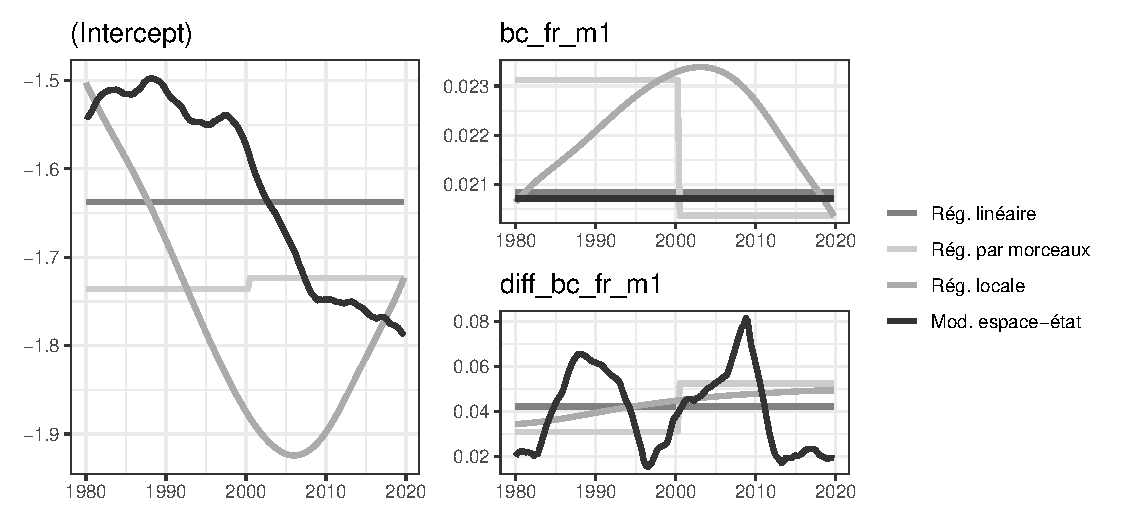
\includegraphics{DT-tvcoef_files/figure-pdf/fig-coef-covid-1.pdf}

}

\end{figure}%

Dans les données ici utilisées, le taux de croissance trimestriel du PIB
est connu jusqu'au 2022T4 alors que les variables explicatives sont
connues jusqu'au 2023T1 :

\begin{Shaded}
\begin{Highlighting}[]
\FunctionTok{tail}\NormalTok{(data\_covid[, }\FunctionTok{c}\NormalTok{(}\StringTok{"growth\_gdp"}\NormalTok{, }\StringTok{"bc\_fr\_m1"}\NormalTok{, }\StringTok{"diff\_bc\_fr\_m1"}\NormalTok{)], }\DecValTok{2}\NormalTok{)}
\end{Highlighting}
\end{Shaded}

\begin{verbatim}
        growth_gdp bc_fr_m1 diff_bc_fr_m1
2022 Q4 0.07510078    102.1          -0.7
2023 Q1         NA    102.0          -0.1
\end{verbatim}

Il est donc possible d'effectuer une prévision sur le dernier trimestre
et nous allons maintenant montrer comment procéder. Le plus simple est
d'effectuer une somme pondérée des variables explicatives avec les
coefficients estimés. Dans cet exemple, les variables explicatives sont
directement calculées dans la base de données en entrée et sont donc
facile à extraire. Lorsque ce n'est pas le cas (par exemple lorsque des
variables retardées ou en différence sont directement calculées dans la
formule de la fonction \texttt{dynlm()}\footnote{ Ce qui aurait pu être
  le cas si le modèle avait été estimé en utilisant le paramètre
  \texttt{formula\ =\ growth\_gdp\ \textasciitilde{}\ bc\_fr\_m1\ +\ diff(bc\_fr\_m1,\ 1)}
  dans la fonction \texttt{dynlm()}.}) il faut alors recalculer toutes
les variables explicatives. La fonction
\texttt{tvCoef::full\_exogeneous\_matrix()} peut aider à effectuer cette
tache et calcule également le régresseur associé à la constante (égal à
1) :

\begin{Shaded}
\begin{Highlighting}[]
\NormalTok{data\_prev }\OtherTok{\textless{}{-}} \FunctionTok{full\_exogeneous\_matrix}\NormalTok{(reg\_lin\_covid)}
\CommentTok{\# On extrait le dernier trimestre :}
\NormalTok{der\_period }\OtherTok{\textless{}{-}} \FunctionTok{tail}\NormalTok{(data\_prev, }\DecValTok{1}\NormalTok{)}
\NormalTok{der\_period}
\end{Highlighting}
\end{Shaded}

\begin{verbatim}
        (Intercept) bc_fr_m1 diff_bc_fr_m1 ind2020T1 ind2020T2 ind2020T3
2023 Q1           1      102          -0.1         0         0         0
        ind2020T4
2023 Q1         0
\end{verbatim}

\begin{Shaded}
\begin{Highlighting}[]
\CommentTok{\# Transformation en numeric pour éviter des erreurs dues au format ts()}
\NormalTok{der\_period }\OtherTok{\textless{}{-}} \FunctionTok{as.numeric}\NormalTok{(der\_period)}
\NormalTok{prev\_reg\_lin }\OtherTok{\textless{}{-}} \FunctionTok{sum}\NormalTok{(}\FunctionTok{coef}\NormalTok{(reg\_lin\_covid) }\SpecialCharTok{*}\NormalTok{ der\_period)}
\CommentTok{\# Pour les autres méthodes on prend les derniers coefficients estimés}
\NormalTok{prev\_reg\_morc }\OtherTok{\textless{}{-}} \FunctionTok{sum}\NormalTok{(}\FunctionTok{tail}\NormalTok{(}\FunctionTok{coef}\NormalTok{(reg\_morc\_covid), }\DecValTok{1}\NormalTok{) }\SpecialCharTok{*}\NormalTok{ der\_period)}
\NormalTok{prev\_reg\_loc }\OtherTok{\textless{}{-}} \FunctionTok{sum}\NormalTok{(}\FunctionTok{tail}\NormalTok{(}\FunctionTok{coef}\NormalTok{(reg\_loc\_covid), }\DecValTok{1}\NormalTok{) }\SpecialCharTok{*}\NormalTok{ der\_period)}
\NormalTok{prev\_ssm }\OtherTok{\textless{}{-}} \FunctionTok{sum}\NormalTok{(}\FunctionTok{tail}\NormalTok{(}\FunctionTok{coef}\NormalTok{(ssm\_covid), }\DecValTok{1}\NormalTok{) }\SpecialCharTok{*}\NormalTok{ der\_period)}
\FunctionTok{round}\NormalTok{(}
  \FunctionTok{c}\NormalTok{(prev\_reg\_lin, prev\_reg\_morc, prev\_reg\_loc, prev\_ssm), }
  \DecValTok{2}\NormalTok{)}
\end{Highlighting}
\end{Shaded}

\begin{verbatim}
[1] 0.49 0.37 0.36 0.36
\end{verbatim}

\section{Comparaison générale}\label{sec-comp-generales}

Dans cette section nous effectuons une comparaison plus détaillée des
différentes méthodes utilisées. Pour cela, nous utilisons 28 modèles de
prévisions des taux de croissance trimestriels de l'industrie
manufacturière et de ses principales sous-branches. Les modèles sont
estimés entre 1992 et 2019 en utilisant des données issues des enquêtes
de conjoncture de l'Insee et de la Banque de France, ainsi que l'Indice
de Production Industrielle des branches étudiées. Parmi ces 28 modèles,
la procédure de Bai et Perron détecte au moins une rupture sur 14
modèles et le test de Hansen conclut à la présence de coefficients
mobiles dans 12 modèles (table~\ref{tbl-nb-models}). Cela permet donc
également de comparer les résultats de la régression locale et de la
modélisation espace-état lorsque les coefficients ne sont pas considérés
comme fixes par les tests étudiés. Dans la suite, nous considérerons
qu'un modèle n'a pas de rupture lorsque le test de Bai et Perron n'en
détecte aucune : dans ce cas, la régression par morceaux donne le même
résultat que la régression linéaire.

\begin{longtable}{l|ccc}

\caption{\label{tbl-nb-models}Nombre de modèles étudiés par branche
d'activité.}

\tabularnewline

\toprule
\multicolumn{1}{l}{} &  & \multicolumn{2}{c}{Avec rupture} \\ 
\cmidrule(lr){3-4}
\multicolumn{1}{l}{} & Total & Bai et Perron & Hansen \\ 
\midrule\addlinespace[2.5pt]
Industrie manufacturière (C) & 3 & 2 & 2 \\ 
Agro–alimentaire (C1) & 7 & 0 & 0 \\ 
Biens d'équipement (C3) & 6 & 4 & 5 \\ 
Matériels de transport (C4) & 6 & 2 & 0 \\ 
Autres industries (C5) & 6 & 6 & 5 \\ 
\midrule 
\midrule 
Total & 28 & 14 & 12 \\ 
\bottomrule

\end{longtable}

Lecture : dans la branche des biens d'équipement (C3), 6 modèles sont
étudiés. Dans 4 de ces modèles la procédure de Bai et Perron conclut à
la présence d'au moins une rupture et le test d'Hansen conclut que les
coefficients sont mobiles dans 5 de ces modèles.

Pour l'estimation des modèles des modèles de régression par morceaux,
nous limitons le nombre maximal de ruptures à 2. La dernière rupture est
détectée en 2011Q4 pour deux modèles de la branche des autres industries
(C5). Les prévisions en hors échantillon sont donc calculées après 2013
afin d'éviter les fortes erreurs autour des ruptures. Pour la régression
locale et la modélisation espace-état, les modèles sont estimés avec les
paramètres par défaut sans chercher à optimiser les modèles (par exemple
en ne fixant pas les coefficients des indicatrices). Ainsi, même si les
estimations pourrait être améliorées, cela permet d'étudier leur qualité
prédictive dans le cas le moins favorable.

Si l'on souhaite comparer les résultats entre les différentes branches,
il est nécessaire de normaliser les erreurs de prévision. Les
indicateurs classiques, tels que l'erreur absolue moyenne en
pourcentage, normalisent en utilisant la variable à prévoir. Cela
nécessite toutefois que ces variables soient positives et non nulles, ce
qui n'est pas le cas des taux de croissance. C'est pourquoi dans cette
section nous utilisons la moyenne absolue des erreurs normalisées ---
\emph{Mean absolute scaled error} (MASE) --- proposée par
\textcite{HYNDMAN2006679} : \[
MASE=moyenne\left(\frac{|{\hat y}_{t} - y_t|}{Q}\right),
\] où \(Q\) est une mesure stable de l'échelle de la série. Pour les
séries non saisonnières, ce qui est ici le cas, nous utilisons : \[
Q=\frac{1}{T-1}\sum_{t=2}^T|y_t-y_{t-1}|.
\]

La table~\ref{tbl-error-table} montre les résultats des MASE associées
différentes méthodes relativement aux prévisions du modèle de régression
linéaire. Dans l'ensemble ce sont les modèles espace-état qui donne les
meilleurs résultats. Pour les modèles où une rupture a été détectée, les
modèles espace état permettent d'améliorer la qualité d'en moyenne 18~\%
par rapport à la régression linéaire (avec un minimum de 6~\%), contre
une amélioration d'en moyenne 12~\% ou 11~\% pour la régression locale
et la régression par morceaux. Hors échantillon, les résultats sont
également améliorés avec la modélisation espace état pour la majorité
des modèles (en moyenne de 7~\% et au maximum de 20~\%) mais sont
dégradés pour 3 des 14 modèles (d'au plus 5~\%). Pour la régression
locale, les résultats sont, dans la majorité des cas (12 modèles sur 14)
identiques ou dégradés par rapport à la régression linéaire (avec une
dégradation d'au plus 17~\%). Pour la régression par morceaux, même si
pour 8 séries les résultats sont améliorées, cette amélioration semble
moins forte qu'avec les modèles espace (au plus 11~\%).

Étonnamment, lorsqu'aucune rupture n'est détectée les modèles
espace-état permettent également d'améliorer les résultats : dans
l'échantillon les erreurs de prévisions sont réduites d'en moyenne 7~\%
et d'au plus 22~\% et ne sont jamais dégradées. Elles sont en revanche
dégradées pour quelques modèles en temps réel (d'au plus 7~\%), elle
sont améliorées pour 3 modèles (jusqu'à 27~\%). Cette instabilité
provient également du fait qu'aucune optimisation n'est faite dans la
spécification des modèles. Toutefois ces résultats suggèrent que les
tests ici présentés pour tester la constance des coefficients ne sont
pas toujours pertinents. Ainsi, \textcite{abs2006} proposent une
procédure de tests basée sur la modélisation espace état (en testant la
significativité de la variance des coefficients estimés).

\begin{longtable}{l|cccccc}

\caption{\label{tbl-error-table}Moyenne absolue des erreurs normalisées
(MASE) rapportée à celle des modèles régression linéaire.}

\tabularnewline

\toprule
\multicolumn{1}{l}{} &  &  &  & \multicolumn{3}{c}{Séries dont MASE} \\ 
\cmidrule(lr){5-7}
\multicolumn{1}{l}{} & Moyenne & Min & Max & < 1 & = 1 & > 1 \\ 
\midrule\addlinespace[2.5pt]
\multicolumn{7}{l}{Sans rupture - Dans l'échantillon} \\ 
\midrule\addlinespace[2.5pt]
Rég. par morceaux & $1,00$ & $1,00$ & $1,00$ & $0$ & $14$ & $0$ \\ 
Rég. locale & $1,00$ & $0,98$ & $1,00$ & $3$ & $11$ & $0$ \\ 
Mod. espace-état & $0,93$ & $0,78$ & $1,00$ & $7$ & $7$ & $0$ \\ 
\midrule\addlinespace[2.5pt]
\multicolumn{7}{l}{Sans rupture - Hors échantillon} \\ 
\midrule\addlinespace[2.5pt]
Rég. par morceaux & $1,00$ & $1,00$ & $1,00$ & $0$ & $14$ & $0$ \\ 
Rég. locale & $1,01$ & $0,99$ & $1,07$ & $1$ & $7$ & $6$ \\ 
Mod. espace-état & $0,99$ & $0,73$ & $1,07$ & $3$ & $7$ & $4$ \\ 
\midrule\addlinespace[2.5pt]
\multicolumn{7}{l}{Avec rupture - Dans l'échantillon} \\ 
\midrule\addlinespace[2.5pt]
Rég. par morceaux & $0,89$ & $0,79$ & $1,00$ & $13$ & $1$ & $0$ \\ 
Rég. locale & $0,88$ & $0,59$ & $1,01$ & $13$ & $0$ & $1$ \\ 
Mod. espace-état & $0,82$ & $0,61$ & $0,94$ & $14$ & $0$ & $0$ \\ 
\midrule\addlinespace[2.5pt]
\multicolumn{7}{l}{Avec rupture - Hors échantillon} \\ 
\midrule\addlinespace[2.5pt]
Rég. par morceaux & $1,00$ & $0,89$ & $1,18$ & $8$ & $1$ & $5$ \\ 
Rég. locale & $1,03$ & $0,91$ & $1,17$ & $2$ & $5$ & $7$ \\ 
Mod. espace-état & $0,93$ & $0,80$ & $1,05$ & $11$ & $0$ & $3$ \\ 
\bottomrule

\end{longtable}

Note : les modèles sans rupture sont ceux où aucune rupture n'est
détectée par la procédure de Bai et Perron.

Lecture : pour les prévisions hors échantillon la modélisation permet,
par rapport à la régression linéaire, le MASE est réduit d'en moyenne de
7~\% pour les modèles avec rupture et de 1~\% pour les modèles sans
rupture. Trois modèles sans rupture sont améliorés grâce à la
modélisation espace-état (avec une réduction maximale de la MASE de
27~\%) et les erreurs de prévisions sont augmentées pour quatre modèles
(avec une hausse maximale de 7~\%).

\section{Conclusion}\label{conclusion}

En conclusion, cette étude montre comment, à partir d'un modèle de
régression linéaire, on peut tester l'hypothèse de constance des
coefficients et relâcher cette hypothèse en implémentant des modèles de
régression par morceaux, de régression mobile et espace-état. Cette
implémentation est facilitée grâce au package \texttt{tvCoef}
(\url{https://github.com/InseeFrLab/tvCoef}) qui accompagne cette étude
et tous les codes associés sont disponibles sous sous
\url{https://github.com/InseeFrLab/DT-tvcoef}.

Lorsque les tests classiques indiquent une non-constance des
coefficients, ces trois méthodes permettent de réduire les erreurs de
prévisions dans l'échantillon (lorsque les coefficients sont estimés sur
l'ensemble des données). Toutefois, ces trois méthodes reposent sur des
hypothèses qui peuvent conduire à des fortes instabilités, notamment si
elles sont utilisées naïvement lors des exercices de prévision en temps
réel (hors échantillon).\\
La régression par morceaux supposent la connaissance de dates de
ruptures : même si des procédures existent pour leur détection
automatique \autocite{bai2003computation}, les instabilités autour de
celles-ci font qu'il est préférable de s'appuyer sur un raisonnement
économique. En effet, si rupture brutale il y a, elle doit pouvoir
s'expliquer et le statisticien devrait pouvoir en trouver la cause.\\
Le paramètre principal de la régression locale est la fenêtre, qui
permet de jouer sur la sensibilité des estimations aux observations
lointaines. Même s'il existe également des procédures de sélection
automatique, celles-ci sont également instables, ce qui conduit, lors
des exercices de prévisions en temps réel, à des erreurs de prévisions
plus élevées que la régression linéaire lorsque la fenêtre n'est pas
fixée.\\
Enfin, dans les modèles espace-état, des instabilités numériques
d'optimisation peuvent conduire à une volatilité dans l'estimation des
variances des coefficients (qui déterminent si le coefficient varie ou
non dans le temps et à quelle vitesse). C'est toutefois la méthode qui
donnent les meilleurs résultats et qui permet dans la majorité des cas
de réduire les erreurs de prévision par rapport à la régression
linéaire, même les tests classiques indiquent une constance des
coefficients !

Même si ces méthodes permettent, par rapport à la régression linéaire,
d'améliorer la qualité des prévisions, elles n'ont pas vocation à
remplacer les modèles existants mais plutôt à les compléter. En effet,
même si dans la majorité des cas les méthodes étudiées permettent de
réduire les erreurs de prévision, cela peut ne pas être le cas sur tous
les trimestres. D'une part la combinaison de prévisions issues de
différents modèles permet généralement d'obtenir une prévision finale
plus précise \autocite[voir par exemple][ pour une revue de
littérature]{WANG20231518} ; d'autre part, l'interprétation économique
et les hypothèses sous-jacentes sont différentes entre chaque modèle :
l'analyse faite de la prévision dépend donc également de la conjoncture
récente.

Cette étude pourrait être étendue de plusieurs manières. Tout d'abord,
les méthodes ici présentées pourraient être améliorées. Par exemple,
pour la régression locale et la modélisation espace-état, on suppose que
les paramètres évoluent à la même vitesse au cours de toute la période
d'estimation (fenêtre fixe et variance fixée). Toutefois, autour des
périodes de crises (comme le COVID-19) on pourrait vouloir ajouter plus
de flexibilités à l'évolution des coefficients (en réduisant la fenêtre
ou en effectuant un choc sur la variance) : cela ajouterait plus de
variabilité dans les estimations mais pourrait permettre de mieux
prendre en compte les changements structurels.\\
Ensuite, d'autres méthodes d'estimations pourraient être utilisées pour
modéliser l'évolution dans le temps des coefficients. Par exemple
\textcite{melard} modélise des variations déterministes des coefficients
(plutôt que stochastiques comme pour les modèles espace-état).\\
Enfin, les modèles auraient également pu être comparés aux modèles à
seuil et modèles à changement de régime markoviens \autocite[voir par
exemple][ pour une revue bibliographique de ces
modèles]{PETROPOULOS2022705} qui peuvent se voir comme des cas
particuliers des méthodes étudiés. En effet, dans les modèles à seuil la
rupture est brutale et dépend du niveau d'une variable exogène et dans
les modèles à changement de régime markoviens, les coefficients
dépendent d'une variable inobservée modélisant la position de l'économie
dans le cycle : la rupture est donc brutale et dépend d'une variable
externe (comme dans la régression locale). \emph{In fine}, le choix
entre toutes ces méthodes se fait surtout sur les hypothèses économiques
que l'on souhaite modéliser.

\appendix

\section{\texorpdfstring{Installation de
\texttt{tvCoef}}{Installation de tvCoef}}\label{installation-de-tvcoef}

Pour utiliser \texttt{tvCoef}, il faut il faut avoir la version 17 de
Java SE (ou une version supérieure).

Pour savoir quelle version de Java est utilisée par R, utiliser le code
suivant :

\begin{Shaded}
\begin{Highlighting}[]
\FunctionTok{library}\NormalTok{(rJava)}
\FunctionTok{.jinit}\NormalTok{()}
\FunctionTok{.jcall}\NormalTok{(}\StringTok{"java/lang/System"}\NormalTok{, }\StringTok{"S"}\NormalTok{, }\StringTok{"getProperty"}\NormalTok{, }\StringTok{"java.runtime.version"}\NormalTok{)}
\end{Highlighting}
\end{Shaded}

Si le résultat n'est pas sous la forme \texttt{"17xxxx"} c'est que vous
n'avez pas Java 17 !

Si l'on a pas cette version d'installée et que l'on n'a pas les droits
d'administrateur pour installer Java, une solution est d'installer une
version portable de Java, par exemple installer une version portable à
partir des liens suivants :

\begin{itemize}
\item
  \href{https://www.azul.com/downloads/\#zulu}{Zulu JDK}
\item
  \href{https://adoptopenjdk.net/}{AdoptOpenJDK}
\item
  \href{https://aws.amazon.com/corretto/}{Amazon Corretto}
\end{itemize}

Pour installer une version portable de java, télécharger par exemple le
fichier \texttt{Windows\ 10\ x64\ Java\ Development\ Kit} disponible sur
\url{https://jdk.java.net/java-se-ri/17}, le dézipper et le mettre par
exemple sous \texttt{""}.

Pour configurer R avec une version portable de Java, trois solutions~:

\begin{enumerate}
\def\labelenumi{\arabic{enumi}.}
\tightlist
\item
  Avant \textbf{avant tout chargement de package nécessitant Java
  (\texttt{rJava}\ldots)} (si vous avez lancé le code précédent,
  relancez donc R) :
\end{enumerate}

\begin{Shaded}
\begin{Highlighting}[]
\CommentTok{\# Si la version portable est installée sous D:/Programmes/jdk{-}17}
\FunctionTok{Sys.setenv}\NormalTok{(}\AttributeTok{JAVA\_HOME=}\StringTok{\textquotesingle{}D:/Programmes/jdk{-}17\textquotesingle{}}\NormalTok{)}
\end{Highlighting}
\end{Shaded}

\begin{enumerate}
\def\labelenumi{\arabic{enumi}.}
\setcounter{enumi}{1}
\tightlist
\item
  Pour éviter de faire cette manipulation à chaque fois que l'on relance
  R, deux solutions~:
\end{enumerate}

\begin{enumerate}
\def\labelenumi{\alph{enumi}.}
\item
  modifier le \texttt{JAVA\_HOME} dans les variables d'environnement de
  Windows (voir
  \url{https://confluence.atlassian.com/doc/setting-the-java_home-variable-in-windows-8895.html}).
\item
  modifier le \texttt{.Renviron} : depuis R lancer le code
  \VERB|\FunctionTok{file.edit}\NormalTok{(}\StringTok{"\textasciitilde{}/.Renviron"}\NormalTok{)}|,
  ajouter dans le fichier le chemin vers la version portable de Java
  comme précédemment
  (\texttt{JAVA\_HOME=\textquotesingle{}D:/Programmes/jdk-17\textquotesingle{}}),
  sauvegarder et relancer R.
\end{enumerate}

Il reste maintenant à installer les packages :

\begin{Shaded}
\begin{Highlighting}[]
\CommentTok{\# Nécessaire pour installer rjd3sts}
\NormalTok{remotes}\SpecialCharTok{::}\FunctionTok{install\_github}\NormalTok{(}\StringTok{"rjdemetra/rjd3toolkit"}\NormalTok{)}
\CommentTok{\# Pour installer rjd3sts (modèles espace{-}état)}
\NormalTok{remotes}\SpecialCharTok{::}\FunctionTok{install\_github}\NormalTok{(}\StringTok{"rjdemetra/rjd3sts"}\NormalTok{)}
\NormalTok{remotes}\SpecialCharTok{::}\FunctionTok{install\_github}\NormalTok{(}\StringTok{"InseeFrLab/tvCoef"}\NormalTok{)}
\end{Highlighting}
\end{Shaded}

Si vous utilisez un ordinateur professionnel, si c'est nécessaire,pensez
à configurer le proxy pour que ces commandes puissent fonctionner (voir
\url{https://www.book.utilitr.org/01_r_insee/fiche-personnaliser-r\#le-fichier-.renviron}).
Pour cela vous pouvez utiliser \texttt{curl::ie\_get\_proxy\_for\_url()}
pour récupérer l'adresse du proxy et ajouter deux variable
\texttt{http\_proxy} et \texttt{https\_proxy} dans les variables
d'environnement (comme précédemment).

\section*{Bibliographie}\label{bibliographie}
\addcontentsline{toc}{section}{Bibliographie}

\printbibliography[heading=none]




\end{document}
